\documentclass[11pt,a4paper]{article}
\usepackage{ifthen}

% ========== MAIN DOCUMENT ENTRY POINT ==========
% This is the main entry point that loads configurations and content separately
% Modify the settings below to customize your document
%
% QUICK START:
% 1. Choose a template OR cover (uncomment one line below)
% 2. Customize the cover content variables
% 3. Enable/disable modules based on your needs
% 4. Compile with: xelatex main.tex

% ========== TEMPLATE AND COVER CONFIGURATION ==========
% 
% IMPORTANT: Choose ONLY ONE option below!
%
% Templates provide both cover page AND document styling (backgrounds, headers, etc.)
% Covers provide ONLY the cover page without affecting document styling
%
% If you're unsure, start with a template - they provide the most complete experience.

% ========== OPTION 1: TEMPLATES (Recommended) ==========
% Templates include professional cover pages + document styling
% Uncomment EXACTLY ONE template line below:
%
% \def\UseTemplate{template1}  % Modern geometric design - Great for tech/marketing docs
% \def\UseTemplate{template2}  % Corporate sidebar design - Perfect for business reports  
% \def\UseTemplate{template3}  % Minimal elegant design - Ideal for academic papers
%
% Template Features:
% - template1: Geometric patterns, modern colors, dynamic backgrounds
% - template2: Professional sidebar, corporate styling, structured layout
% - template3: Clean minimal design, elegant typography, academic focus

% ========== OPTION 2: STANDALONE COVERS ==========
% Use ONLY if you want a cover page without template styling
% Uncomment EXACTLY ONE cover line below (ONLY if no template selected above):
%
% \def\UseCover{cover1}   % Modern gradient design - Colorful and dynamic
\def\UseCover{cover2}   % Professional layout - Clean business style
% \def\UseCover{cover3}   % Clean minimal design - Simple and elegant
% \def\UseCover{cover4}   % Corporate style - Formal business appearance
% \def\UseCover{cover5}   % Academic format - Traditional academic layout
% \def\UseCover{cover6}   % Creative design - Artistic and unique
% \def\UseCover{cover7}   % Technical report - Engineering/technical focus
% \def\UseCover{cover8}   % Elegant filigree design - Ornate academic style
% \def\UseCover{cover9}   % Modern minimalist design - Clean and simple
% \def\UseCover{cover10}  % Contemporary blocks design - Colorful geometric
%
% Note: Covers only affect the first page. The rest of your document will use basic styling.
%
% SPECIAL REQUIREMENTS:
% - Cover1: Requires TikZ libraries (positioning, shapes.geometric, decorations.pathmorphing, shadows.blur, backgrounds, calc)
% - Cover2: Requires fp package for mathematical calculations
% - Cover3: Requires TikZ libraries (positioning, shapes, decorations.pathmorphing, patterns, calc)
% - Cover4: Requires datetime2 package and TikZ libraries (positioning, shapes, decorations.pathmorphing, calc)
% - Cover5: Requires datetime2 package and TikZ libraries (positioning, shapes, decorations.pathmorphing, patterns, calc)
% - Cover6: Requires TikZ libraries (positioning, shapes, decorations.pathmorphing, patterns, calc, fadings)
% - Cover7: Requires TikZ libraries (positioning, calc)
%
% All required packages are automatically loaded by config.tex when covers are used.

% ========== COVER CONTENT CUSTOMIZATION ==========
% These variables are used by both templates and covers
% Customize them to match your document:
%
\newcommand{\CoverTitle}{Your Document Title}        % Main title on cover page
\newcommand{\CoverSubtitle}{Document Subtitle}       % Subtitle/description
\newcommand{\CoverYear}{2024}                        % Year or date
\newcommand{\CoverRecipient}{Recipient Name}         % Who is this document for?
\newcommand{\CoverPreparer}{Author Name}             % Who created this document?
%
% Example for a business report:
% \newcommand{\CoverTitle}{Q4 2024 Sales Analysis}
% \newcommand{\CoverSubtitle}{Regional Performance Review}
% \newcommand{\CoverYear}{December 2024}
% \newcommand{\CoverRecipient}{Executive Team}
% \newcommand{\CoverPreparer}{Sales Analytics Department}

% ========== ADVANCED COVER CUSTOMIZATION ==========
% Some covers support additional customization options.
% Uncomment and modify these if you want to override the defaults:
%
% For Cover3 (Modern Corporate):
% \renewcommand{\CompanyPlaceholder}{Your Company Name}
% \renewcommand{\DepartmentPlaceholder}{Your Department}
%
% For Cover4 (Academic):
% \renewcommand{\InstitutionPlaceholder}{Your Institution}
% \renewcommand{\AbstractPlaceholder}{Your abstract text here...}
% \renewcommand{\KeywordsPlaceholder}{keyword1, keyword2, keyword3}
%
% For Cover5 (Technical Blueprint):
% \renewcommand{\DocumentIDPlaceholder}{DOC-2024-001}
% \renewcommand{\RevisionPlaceholder}{B}
%
% For Cover7 (Professional):
% \renewcommand{\ContactPlaceholder}{your.email@company.com}
%
% NOTE: This system uses \def to ensure proper template/cover selection.
% If you get compilation errors, ensure only ONE template OR cover is uncommented.

% ========== MODULE CONFIGURATION ==========
% 
% Modules are optional LaTeX packages that add specific features to your document.
% Enable ONLY the modules you actually need to keep compilation fast and clean.
%
% PERFORMANCE TIP: Each enabled module increases compilation time:
% - Basic (4 modules): 8-12 seconds
% - Selective (6-7 modules): 15-25 seconds  
% - Full (all modules): 25-35 seconds
%
% Set to 'true' to enable, 'false' to disable:

\newcommand{\EnableAdvancedTypography}{true}   % Drop caps, advanced fonts, letter spacing
                                               % Use for: Professional documents, marketing materials
                                               
\newcommand{\EnableMathematics}{true}          % Equations, theorems, mathematical symbols
                                               % Use for: Academic papers, technical documents, research
                                               
\newcommand{\EnableTables}{true}               % Enhanced table formatting, colors, multi-page tables
                                               % Use for: Data reports, comparisons, structured information
                                               
\newcommand{\EnableBoxes}{true}                % Info boxes, alerts, callouts, warnings
                                               % Use for: Almost all documents (highly recommended)
                                               
\newcommand{\EnableLists}{false}               % Enhanced lists, task lists, priority indicators
                                               % Use for: Project plans, checklists, structured content
                                               
\newcommand{\EnableCode}{false}                % Syntax highlighting, code blocks, programming examples
                                               % Use for: Technical documentation, programming guides
                                               
\newcommand{\EnableImages}{false}              % Advanced image handling, positioning, effects
                                               % Use for: Visual documents, reports with graphics
                                               
\newcommand{\EnableAlgorithms}{false}          % Pseudocode, algorithm formatting, flowcharts
                                               % Use for: Computer science papers, technical specifications
                                               
\newcommand{\EnableReferences}{false}          % Bibliography, citations, cross-references
                                               % Use for: Academic papers, research documents
%
% COMMON COMBINATIONS:
%
% Academic Paper:
% Mathematics=true, References=true, Algorithms=true, Boxes=true
%
% Business Report:  
% Tables=true, Boxes=true, Images=true, AdvancedTypography=true
%
% Technical Documentation:
% Code=true, Mathematics=true, Tables=true, Boxes=true
%
% Quick Draft:
% Boxes=true (minimal setup for fast compilation)

% ========== LOAD CONFIGURATION ==========
% This loads the core LaTeX configuration and all enabled modules
% DO NOT MODIFY - this handles all the complex package loading
% ========== CORE CONFIGURATION ==========
% Lightweight core configuration for basic LaTeX documents
% ========== ESSENTIAL PACKAGES ==========
% Instructions: These packages handle font setup and character encoding
% Keep these as-is unless you need different fonts
\usepackage{inputenc}
\usepackage[T1]{fontenc}
\usepackage{lmodern}
\usepackage{ifthen}
\usepackage{geometry}
\usepackage{fontspec}
\usepackage{setspace}
\usepackage{xcolor}
\usepackage{morefloats}
\usepackage[table]{xcolor}
% Load TikZ for covers and templates
\usepackage{tikz}
\usepackage{eso-pic}
% Load fp package for mathematical calculations (needed by some covers)
\usepackage{fp}
% Load datetime2 package for date formatting (needed by covers 4 and 5)
\usepackage{datetime2}
\ifdefined\pdftexversion
  \usepackage{microtype}
\fi

% ========== BASIC PAGE LAYOUT ==========
\geometry{
    top=1.2in,
    bottom=1.2in,
    left=1.1in,
    right=1.1in,
    headheight=14pt,
    headsep=0.3in,
    footskip=0.45in
}

% ========== BASIC COLORS ==========
% Essential colors only - load brand_colors.tex if it exists
\definecolor{primary}{HTML}{0F172A}
\definecolor{secondary}{HTML}{334155}
\definecolor{accent}{HTML}{2563EB}
\definecolor{success}{HTML}{059669}
\definecolor{warning}{HTML}{D97706}
\definecolor{background}{HTML}{F8FAFC}
\definecolor{border}{HTML}{E2E8F0}
\definecolor{textgray}{HTML}{64748B}

% Try to load brand colors if available
\IfFileExists{brand_colors.tex}{
    % ========== BRAND COLORS ==========
% Define your brand colors here to maintain consistent branding across your document
% These colors will be used throughout the document for various elements

% Primary Brand Colors - CUSTOMIZE THESE
\definecolor{brandPrimary}{HTML}{2563EB}    % Primary brand color
\definecolor{brandSecondary}{HTML}{4F46E5}  % Secondary brand color
\definecolor{brandAccent}{HTML}{10B981}     % Accent color for highlights and emphasis

% Text Colors - Derived from brand colors
\definecolor{primary}{HTML}{0F172A}         % Main text color
\definecolor{secondary}{HTML}{334155}       % Secondary text color
\definecolor{accent}{HTML}{2563EB}          % Links and highlights (defaults to brandPrimary)

% UI Element Colors - These should work well with your brand colors
\definecolor{lightaccent}{HTML}{3B82F6}     % Lighter accent variant
\definecolor{success}{HTML}{059669}         % Success/positive elements
\definecolor{warning}{HTML}{D97706}         % Warning/attention elements
\definecolor{background}{HTML}{F8FAFC}      % Light background for boxes
\definecolor{border}{HTML}{E2E8F0}          % Borders and lines
\definecolor{textgray}{HTML}{64748B}        % Muted text
\definecolor{lightgray}{HTML}{F1F5F9}       % Table alternating rows

% Code Colors
\definecolor{codebg}{HTML}{F8F8F8}          % Code block background
\definecolor{codecomment}{HTML}{6A737D}     % Code comments
\definecolor{codestring}{HTML}{032F62}      % Code strings
\definecolor{codekey}{HTML}{D73A49}         % Code keywords

% Table Colors
\definecolor{cardbg}{HTML}{F7F9FC}          % Card background color
\definecolor{headerbg}{HTML}{4A90E2}        % Table header background (defaults to a shade of brandPrimary)
\definecolor{headertext}{HTML}{FFFFFF}      % Text color for table headers
\definecolor{rowalt}{HTML}{F1F4F9}          % Alternating row color
\definecolor{frameborder}{HTML}{D3DCE6}     % Border color for frames

% ========== COLOR CASCADE SYSTEM ==========
% This automatically adjusts certain colors based on your brand colors
% Uncomment and adjust these lines to automatically derive colors from your brand colors

% Table header background from brand primary
\colorlet{headerbg}{brandPrimary}

% Accent color from brand primary
\colorlet{accent}{brandPrimary}

% Light accent as a lighter shade of brand primary
\colorlet{lightaccent}{brandPrimary!75}

% Success color from brand accent
\colorlet{success}{brandAccent}

% Border color from brand colors
\colorlet{border}{brandPrimary!20}

% Frame border from brand secondary
\colorlet{frameborder}{brandSecondary!30}

% ========== END COLOR CASCADE SYSTEM ========== 
    \typeout{^^J INFO: Loaded custom brand colors from brand_colors.tex^^J}
}{
    \typeout{^^J INFO: Using basic colors (brand_colors.tex not found)^^J}
}

% ========== BASIC TYPOGRAPHY ==========
\setlength{\parindent}{0pt}
\setlength{\parskip}{8pt plus 2pt minus 1pt}

% Basic text commands
\newcommand{\brandname}[1]{\textsc{#1}}
\newcommand{\productname}[1]{\textbf{#1}}

% ========== CONDITIONAL LOADING SYSTEM ==========
% Define flags for optional features (set these before loading config-core.tex)
\providecommand{\EnableAdvancedTypography}{false}
\providecommand{\EnableMathematics}{false}
\providecommand{\EnableTables}{false}
\providecommand{\EnableBoxes}{false}
\providecommand{\EnableLists}{false}
\providecommand{\EnableCode}{false}
\providecommand{\EnableImages}{false}
\providecommand{\EnableAlgorithms}{false}
\providecommand{\EnableReferences}{false}

% Load additional modules based on flags
\ifthenelse{\equal{\EnableAdvancedTypography}{true}}{
    % ========== ADVANCED TYPOGRAPHY MODULE ==========
% Load this module only when advanced typography features are needed

% Advanced typography packages
\usepackage{fontspec}
\usepackage{setspace}
% Only load microtype for pdfTeX (not XeTeX/LuaTeX)
\ifdefined\pdftexversion
    \usepackage{microtype}
\fi
\usepackage{soul}
\usepackage{ragged2e}
\usepackage{textcase}
\usepackage{relsize}
\usepackage{scalefnt}
\usepackage{lettrine}
\usepackage[english]{babel}
\usepackage[autostyle=true,english=american]{csquotes}
\usepackage[all]{nowidow}
\usepackage{needspace}

% Font setup with Inter (if available)
\IfFontExistsTF{Inter}{
    \setmainfont{Inter}[
        UprightFont = *-Regular,
        BoldFont = *-SemiBold,
        ItalicFont = *-Italic,
        BoldItalicFont = *-SemiBoldItalic,
        LetterSpace = 3.0
    ]
    \setsansfont{Inter}[
        UprightFont = *-Regular,
        BoldFont = *-SemiBold,
        ItalicFont = *-Italic,
        BoldItalicFont = *-SemiBoldItalic,
        LetterSpace = 3.0
    ]
}{
    \typeout{^^J WARNING: Inter font not found, using default fonts^^J}
}

% Enhanced brand text macros
\renewcommand{\brandname}[1]{{\addfontfeatures{LetterSpace=12.0}\textsc{#1}}}
\renewcommand{\productname}[1]{{\addfontfeatures{LetterSpace=8.0}\textbf{#1}}}

% Line spacing commands
\newcommand{\setSpacingSingle}{\setstretch{1.0}}
\newcommand{\setSpacingOneHalf}{\setstretch{1.5}}
\newcommand{\setSpacingDouble}{\setstretch{2.0}}
\newcommand{\customspacing}[1]{\setstretch{#1}}

% Text decoration commands
\newcommand{\textunderline}[1]{\underline{#1}}
\newcommand{\textstrikeout}[1]{\st{#1}}
\newcommand{\texthi}[2][yellow]{\colorbox{#1}{#2}}

% Letter spacing adjustments
\newcommand{\wide}[1]{\so{#1}}
\newcommand{\wider}[1]{\sowide{#1}}
\newcommand{\narrow}[1]{\sonormal{#1}}
\newcommand{\letterspace}[2][100]{{\addfontfeatures{LetterSpace=#1}#2}}

% Font size adjustments
\newcommand{\textsm}[1]{\textsmaller{#1}}
\newcommand{\textlg}[1]{\textlarger{#1}}

% Case transformation
\newcommand{\uppercased}[1]{\MakeTextUppercase{#1}}
\newcommand{\lowercased}[1]{\MakeTextLowercase{#1}}

% Text alignment
\newcommand{\justifiedtext}{\justify}
\newcommand{\leftalignedtext}{\raggedright}
\newcommand{\rightalignedtext}{\raggedleft}
\newcommand{\centeredtext}{\centering}

% Drop cap configuration
\renewcommand{\LettrineFontHook}{\color{accent}\bfseries}
\setcounter{DefaultLines}{3}
\renewcommand{\DefaultLoversize}{0.1}
\renewcommand{\DefaultLraise}{0}

% Typography fine-tuning
\setlength{\emergencystretch}{3em}
\hyphenpenalty=500
\clubpenalty=10000
\widowpenalty=10000

% Microtype setup (only for pdfTeX)
\ifdefined\pdftexversion
    \microtypesetup{
        activate=true,
        final=true,
        factor=1100
    }
\fi

% Smart quotes setup
\MakeOuterQuote{"}

% Font feature control
\newcommand{\withfeatures}[2]{{\addfontfeatures{#1}#2}}

    \typeout{^^J INFO: Loaded advanced typography module^^J}
}{}

\ifthenelse{\equal{\EnableMathematics}{true}}{
    % ========== MATHEMATICS MODULE ==========
% Load this module only when mathematical typesetting is needed

% Core math packages
\usepackage{amsmath}
\usepackage{amssymb}
\usepackage{fixmath}
\usepackage{siunitx}
\usepackage{mathtools}
\usepackage{empheq}
\usepackage{cases}
\usepackage{amsthm}
\usepackage{stmaryrd}
\usepackage{textcomp}
\usepackage{physics}
\usepackage{tensor}
\usepackage{braket}
\usepackage{cancel}

% Configure siunitx
\sisetup{
    group-separator={,},
    group-minimum-digits=4,
    detect-weight=true,
    detect-family=true
}

% Define common units
\DeclareSIUnit\USD{\$}
\DeclareSIUnit\hour{h}
\DeclareSIUnit\year{yr}

% Theorem environments
\theoremstyle{definition}
\newtheorem{definition}{Definition}[section]
\newtheorem{theorem}{Theorem}[section]
\newtheorem{lemma}[theorem]{Lemma}
\newtheorem{corollary}[theorem]{Corollary}
\newtheorem{proposition}[theorem]{Proposition}
\newtheorem{example}{Example}[section]

\theoremstyle{remark}
\newtheorem{remark}{Remark}[section]
\newtheorem{note}{Note}[section]

% Math colors
\definecolor{mathblue}{RGB}{0,82,155}
\definecolor{mathred}{RGB}{204,0,0}
\definecolor{mathgreen}{RGB}{0,128,0}
\definecolor{mathpurple}{RGB}{128,0,128}

% Common mathematical sets
\newcommand{\R}{\mathbb{R}}
\newcommand{\C}{\mathbb{C}}
\newcommand{\N}{\mathbb{N}}
\newcommand{\Z}{\mathbb{Z}}
\newcommand{\Q}{\mathbb{Q}}
\newcommand{\F}{\mathbb{F}}

% Enhanced derivatives
\renewcommand{\d}{\mathrm{d}}
\newcommand{\dt}{\frac{\d}{\d t}}
\newcommand{\dx}{\frac{\d}{\d x}}
\newcommand{\dy}{\frac{\d}{\d y}}
\newcommand{\dz}{\frac{\d}{\d z}}
\newcommand{\prt}{\partial}
\newcommand{\pdx}[1]{\frac{\partial #1}{\partial x}}
\newcommand{\pdy}[1]{\frac{\partial #1}{\partial y}}
\newcommand{\pdz}[1]{\frac{\partial #1}{\partial z}}
\newcommand{\pdt}[1]{\frac{\partial #1}{\partial t}}

% Vector calculus
\providecommand{\grad}{\nabla}
\providecommand{\divg}{\nabla \cdot}
\providecommand{\curl}{\nabla \times}
\providecommand{\lapl}{\nabla^2}

% Vectors and matrices
\newcommand{\vect}[1]{\mathbf{#1}}
\newcommand{\mat}[1]{\mathbf{#1}}
\newcommand{\T}{\mathsf{T}}

% Probability and statistics
\newcommand{\prob}[1]{\mathrm{P}\left(#1\right)}
\newcommand{\E}[1]{\mathrm{E}\left[#1\right]}
\renewcommand{\var}[1]{\mathrm{Var}\left(#1\right)}
\newcommand{\cov}[1]{\mathrm{Cov}\left(#1\right)}
\newcommand{\normal}{\mathcal{N}}
\newcommand{\uniform}{\mathcal{U}}

% Math operators
\providecommand{\tr}{\operatorname{tr}}
\providecommand{\diag}{\operatorname{diag}}
\providecommand{\rank}{\operatorname{rank}}
\newcommand{\sign}{\operatorname{sign}}
\providecommand{\lcm}{\operatorname{lcm}}
\providecommand{\gcd}{\operatorname{gcd}}

% Boxed equations
\newcommand{\boxedeq}[1]{\begin{empheq}[box=\fbox]{equation}#1\end{empheq}}
\newcommand{\colorboxedeq}[2]{\begin{empheq}[box={\fcolorbox{#1}{white}}]{equation}#2\end{empheq}}

    \typeout{^^J INFO: Loaded mathematics module^^J}
}{}

\ifthenelse{\equal{\EnableTables}{true}}{
    % ========== TABLES MODULE ==========
% Load this module only when advanced table features are needed

% Table packages
\usepackage{booktabs}
\usepackage{tabularx}
\usepackage{caption}
\usepackage{longtable}
\usepackage{array}
\usepackage{multirow}

% Define enhanced column types
\newcolumntype{L}[1]{>{\raggedright\arraybackslash}p{#1}}
\newcolumntype{C}[1]{>{\centering\arraybackslash}p{#1}}
\newcolumntype{R}[1]{>{\raggedleft\arraybackslash}p{#1}}
\newcolumntype{N}{>{\raggedleft\arraybackslash}X}

% Table styling
\captionsetup{font=small, labelfont=bf, labelsep=colon}

% Additional table colors (if not already defined)
\providecommand{\definecolor}[3]{}
\definecolor{cardbg}{HTML}{F7F9FC}
\definecolor{headerbg}{HTML}{4A90E2}
\definecolor{headertext}{HTML}{FFFFFF}
\definecolor{rowalt}{HTML}{F1F4F9}
\definecolor{frameborder}{HTML}{D3DCE6}

    \typeout{^^J INFO: Loaded tables module^^J}
}{}

\ifthenelse{\equal{\EnableBoxes}{true}}{
    % ========== BOXES MODULE ==========
% Load this module only when callout boxes are needed

% Required packages
\usepackage{tikz}
\usetikzlibrary{shadows}
\usepackage[most]{tcolorbox}

% Info box style - use for general information
\newtcolorbox{infobox}[1][]{
    colback=background,
    colframe=accent,
    coltext=primary,
    boxrule=1pt,
    arc=3pt,
    left=12pt,
    right=12pt,
    top=8pt,
    bottom=8pt,
    enhanced,
    drop shadow,
    fonttitle=\bfseries\sffamily\color{white},
    title style={left color=accent, right color=accent!80!black},
    attach boxed title to top left={xshift=8pt, yshift=-2pt},
    #1
}

% Alert box style - use for cautions and important notes
\newtcolorbox{alertbox}[1][]{
    colback=warning!5,
    colframe=warning,
    coltext=primary,
    boxrule=1pt,
    arc=3pt,
    left=12pt,
    right=12pt,
    top=8pt,
    bottom=8pt,
    enhanced,
    drop shadow,
    fonttitle=\bfseries\sffamily\color{white},
    title style={left color=warning, right color=warning!80!black},
    attach boxed title to top left={xshift=8pt, yshift=-2pt},
    #1
}

% Success box style - use for positive highlights
\newtcolorbox{successbox}[1][]{
    colback=success!5,
    colframe=success,
    coltext=primary,
    boxrule=1pt,
    arc=3pt,
    left=12pt,
    right=12pt,
    top=8pt,
    bottom=8pt,
    enhanced,
    drop shadow,
    fonttitle=\bfseries\sffamily\color{white},
    title style={left color=success, right color=success!80!black},
    attach boxed title to top left={xshift=8pt, yshift=-2pt},
    #1
}

% Icon-enhanced boxes (optional - loads fontawesome and awesomebox)
\IfFileExists{fontawesome5.sty}{
    \usepackage{fontawesome5}
    \IfFileExists{awesomebox.sty}{
        \usepackage{awesomebox}
        \typeout{^^J INFO: Loaded icon-enhanced boxes (fontawesome5 + awesomebox)^^J}
    }{
        \typeout{^^J WARNING: awesomebox package not found, icon boxes unavailable^^J}
    }
}{
    \typeout{^^J WARNING: fontawesome5 package not found, icon boxes unavailable^^J}
}

% Logo-enhanced boxes (optional - loads bclogo)
\IfFileExists{bclogo.sty}{
    \usepackage{bclogo}
    \typeout{^^J INFO: Loaded logo-enhanced boxes (bclogo)^^J}
}{
    \typeout{^^J WARNING: bclogo package not found, logo boxes unavailable^^J}
}

    \typeout{^^J INFO: Loaded boxes module^^J}
}{}

\ifthenelse{\equal{\EnableLists}{true}}{
    % ========== LISTS MODULE ==========
% Load this module only when enhanced list features are needed

% List customization package
\usepackage{enumitem}

% Basic list styling
\setlist[itemize,1]{
    leftmargin=18pt,
    itemsep=3pt plus 1pt minus 1pt,
    parsep=0pt,
    topsep=6pt plus 2pt minus 2pt,
    label=\color{accent}$\bullet$
}
\setlist[itemize,2]{
    leftmargin=16pt,
    itemsep=2pt,
    parsep=0pt,
    topsep=3pt,
    label=\color{secondary}$\circ$
}
\setlist[itemize,3]{
    leftmargin=14pt,
    itemsep=1pt,
    parsep=0pt,
    topsep=2pt,
    label=\color{textgray}{\scriptsize$\blacksquare$}
}

% Enhanced enumerate styling
\setlist[enumerate,1]{
    leftmargin=22pt,
    itemsep=3pt plus 1pt minus 1pt,
    parsep=0pt,
    topsep=6pt plus 2pt minus 2pt,
    label=\color{accent}\arabic*.
}
\setlist[enumerate,2]{
    leftmargin=20pt,
    itemsep=2pt,
    parsep=0pt,
    topsep=3pt,
    label=\color{secondary}(\alph*)
}
\setlist[enumerate,3]{
    leftmargin=18pt,
    itemsep=1pt,
    parsep=0pt,
    topsep=2pt,
    label=\color{textgray}\roman*.
}

% Description list styling
\setlist[description]{
    font=\normalfont\color{accent}\bfseries,
    labelwidth=2cm,
    leftmargin=2.5cm,
    itemsep=4pt,
    parsep=0pt
}

% TikZ bullets for professional styling
\usepackage{tikz}
\newcommand{\tikzbullet}[1]{%
    \tikz[baseline=-0.7ex]\node[circle,fill=#1,inner sep=1.5pt]{};%
}

% Compact and expanded list variants
\newenvironment{compactlist}
    {\begin{itemize}[nosep]}
    {\end{itemize}}

\newenvironment{expandedlist}
    {\begin{itemize}[itemsep=8pt,parsep=4pt]}
    {\end{itemize}}

% Task lists with icons (requires fontawesome5)
\IfFileExists{fontawesome5.sty}{
    \usepackage{fontawesome5}
    
    \newlist{tasklist}{itemize}{1}
    \setlist[tasklist]{
        leftmargin=20pt,
        label=\color{success}\faCheck,
        itemsep=4pt,
        parsep=2pt
    }
    
    \newlist{pendingtask}{itemize}{1}
    \setlist[pendingtask]{
        leftmargin=20pt,
        label=\color{warning}\faHourglass,
        itemsep=4pt,
        parsep=2pt
    }
    
    \newlist{failedtask}{itemize}{1}
    \setlist[failedtask]{
        leftmargin=20pt,
        label=\color{accent}\faTimes,
        itemsep=4pt,
        parsep=2pt
    }
    
    % Priority list environments
    \newlist{highpriority}{itemize}{1}
    \setlist[highpriority]{
        leftmargin=20pt,
        label=\color{accent}\faExclamationCircle,
        itemsep=4pt
    }
    
    \newlist{mediumpriority}{itemize}{1}
    \setlist[mediumpriority]{
        leftmargin=20pt,
        label=\color{warning}\faExclamation,
        itemsep=4pt
    }
    
    \newlist{lowpriority}{itemize}{1}
    \setlist[lowpriority]{
        leftmargin=20pt,
        label=\color{success}\faInfoCircle,
        itemsep=4pt
    }
    
    \typeout{^^J INFO: Loaded task and priority lists (fontawesome5)^^J}
}{
    \typeout{^^J WARNING: fontawesome5 not found, task lists unavailable^^J}
}

    \typeout{^^J INFO: Loaded lists module^^J}
}{}

\ifthenelse{\equal{\EnableCode}{true}}{
    % ========== CODE MODULE ==========
% Load this module only when code listings are needed

% Code colors
\definecolor{codebg}{HTML}{F8F8F8}
\definecolor{codecomment}{HTML}{6A737D}
\definecolor{codestring}{HTML}{032F62}
\definecolor{codekey}{HTML}{D73A49}

% Basic code listings
\usepackage{listings}
\lstset{
    basicstyle=\ttfamily\small,
    backgroundcolor=\color{codebg},
    commentstyle=\color{codecomment},
    keywordstyle=\color{codekey}\bfseries,
    stringstyle=\color{codestring},
    numbers=left,
    numberstyle=\tiny\color{textgray},
    numbersep=10pt,
    tabsize=4,
    breaklines=true,
    breakatwhitespace=false,
    frame=single,
    rulecolor=\color{border},
    framesep=8pt,
    showstringspaces=false
}

% Advanced syntax highlighting with minted (optional)
\IfFileExists{minted.sty}{
    \usepackage{minted}
    \setminted{
        style=default,
        bgcolor=codebg,
        linenos=true,
        breaklines=true,
        tabsize=4,
        fontsize=\small,
        frame=single,
        framesep=8pt
    }
    \typeout{^^J INFO: Loaded advanced syntax highlighting (minted)^^J}
}{
    \typeout{^^J WARNING: minted package not found, using basic listings only^^J}
}

    \typeout{^^J INFO: Loaded code module^^J}
}{}

\ifthenelse{\equal{\EnableImages}{true}}{
    % ========== IMAGES MODULE ==========
% Load this module only when advanced image features are needed

% Image packages
\usepackage{graphicx}
\usepackage[export,graphics,noclipbox]{adjustbox}
\usepackage{varwidth}
\usepackage{tikz}

% Create fallback box for missing images
\newsavebox{\imagefallbackbox}

% Command for images with fallback text
\newcommand{\imageWithFallback}[4][]{%
  \begingroup
  \sbox{\imagefallbackbox}{%
    \begin{varwidth}{\textwidth}
      \centering
      \textcolor{textgray}{\textbf{#4}}
    \end{varwidth}
  }%
  \IfFileExists{#2}{%
    \includegraphics[#1,width=#3]{#2}%
  }{%
    \fcolorbox{border}{background}{%
      \begin{minipage}[c][0.75\ht\imagefallbackbox][c]{#3}
        \centering
        \textcolor{textgray}{\faImage}\\[0.3em]
        \usebox{\imagefallbackbox}
      \end{minipage}%
    }%
  }%
  \endgroup
}

% Rectangular image with border
\newcommand{\rectImage}[5][]{%
  \begin{figure}[htbp]
    \centering
    \fbox{\imageWithFallback[#1]{#2}{#3}{#5}}
    \ifx&#4&%
    \else
      \caption{#4}
    \fi
  \end{figure}
}

% Rounded corner image
\newcommand{\roundedImage}[6][]{%
  \begin{figure}[htbp]
    \centering
    \begin{tikzpicture}
      \node[inner sep=0pt] (image) {%
        \imageWithFallback[#1]{#2}{#3}{#6}%
      };
      \begin{scope}
        \clip[rounded corners=#4] (image.south west) rectangle (image.north east);
        \node[inner sep=0pt] {\imageWithFallback[#1]{#2}{#3}{#6}};
      \end{scope}
    \end{tikzpicture}
    \ifx&#5&%
    \else
      \caption{#5}
    \fi
  \end{figure}
}

% Circular image
\newcommand{\circularImage}[5][]{%
  \begin{figure}[htbp]
    \centering
    \begin{tikzpicture}
      \node[inner sep=0pt] (image) {%
        \imageWithFallback[#1]{#2}{#3}{#5}%
      };
      \begin{scope}
        \clip (image.center) circle (#3/2);
        \node[inner sep=0pt] {\imageWithFallback[#1]{#2}{#3}{#5}};
      \end{scope}
    \end{tikzpicture}
    \ifx&#4&%
    \else
      \caption{#4}
    \fi
  \end{figure}
}

% Image with drop shadow
\newcommand{\shadowImage}[5][]{%
  \begin{figure}[htbp]
    \centering
    \begin{tikzpicture}
      \node[inner sep=0pt, drop shadow={shadow xshift=2pt, shadow yshift=-2pt, opacity=0.5}] {%
        \imageWithFallback[#1]{#2}{#3}{#5}%
      };
    \end{tikzpicture}
    \ifx&#4&%
    \else
      \caption{#4}
    \fi
  \end{figure}
}

% Full-width responsive image
\newcommand{\fullwidthImage}[5][]{%
  \begin{figure}[htbp]
    \centering
    \makebox[\textwidth][c]{%
      \imageWithFallback[#1,height=#3,width=\textwidth,keepaspectratio]{#2}{\textwidth}{#5}%
    }
    \ifx&#4&%
    \else
      \caption{#4}
    \fi
  \end{figure}
}

    \typeout{^^J INFO: Loaded images module^^J}
}{}

\ifthenelse{\equal{\EnableAlgorithms}{true}}{
    % ========== ALGORITHMS MODULE ==========
% Load this module only when algorithm typesetting is needed

% Algorithm package
\usepackage[ruled,vlined]{algorithm2e}
\SetAlgoLined
\SetAlgoSkip{medskip}
\SetAlFnt{\footnotesize\sffamily}
\renewcommand{\algorithmcfname}{Algorithm}

    \typeout{^^J INFO: Loaded algorithms module^^J}
}{}

\ifthenelse{\equal{\EnableReferences}{true}}{
    % ========== REFERENCES MODULE ==========
% Load this module only when advanced references are needed

% Reference management packages
\usepackage[
    backend=biber,
    style=authoryear,
    sorting=nyt,
    maxbibnames=99,
    giveninits=true
]{biblatex}

% Hyperref and cross-references (order matters!)
\usepackage{hyperref}
\hypersetup{
    colorlinks=true,
    linkcolor=accent,
    urlcolor=accent,
    citecolor=accent,
    filecolor=accent,
    bookmarks=true,
    bookmarksopen=true,
    bookmarksnumbered=true,
    pdfstartview=FitH,
    pdfpagelayout=SinglePage
}

\usepackage{nameref}
\usepackage{varioref}
\usepackage{cleveref}

% Label formats
\labelformat{figure}{Figure~#1}
\labelformat{table}{Table~#1}
\labelformat{equation}{Equation~#1}
\labelformat{section}{Section~#1}

% Cleveref names
\crefname{figure}{Figure}{Figures}
\crefname{table}{Table}{Tables}
\crefname{equation}{Equation}{Equations}
\crefname{section}{Section}{Sections}

    \typeout{^^J INFO: Loaded references module^^J}
}{}

% ========== BASIC SECTION STYLING ==========
\usepackage{titlesec}
\titleformat{\section}
    {\color{primary}\fontsize{16}{20}\bfseries\sffamily}
    {\color{accent}\thesection}
    {1em}
    {}
    [\vspace{2pt}\color{border}\hrule height 0.8pt\vspace{6pt}]

\titleformat{\subsection}
    {\color{primary}\fontsize{14}{18}\bfseries\sffamily}
    {\color{accent}\thesubsection}
    {0.8em}
    {}

\titlespacing*{\section}{0pt}{20pt plus 4pt minus 2pt}{8pt plus 2pt minus 2pt}
\titlespacing*{\subsection}{0pt}{16pt plus 3pt minus 2pt}{6pt plus 2pt minus 1pt}

% ========== BASIC HEADERS AND FOOTERS ==========
\usepackage{fancyhdr}
\usepackage{lastpage}
\pagestyle{fancy}
\fancyhf{}
\renewcommand{\headrulewidth}{0.5pt}
\renewcommand{\footrulewidth}{0pt}
\fancyhead[L]{\color{textgray}\small\sffamily Your Document Title Here}
\fancyhead[R]{\color{textgray}\small\sffamily\thepage}
\fancyfoot[C]{\color{textgray}\footnotesize\sffamily Page \thepage{} of \pageref{LastPage}}

% ========== DOCUMENT METADATA ==========
\usepackage{titling}
\pretitle{
    \begin{center}
    \vspace{0.5in}
    \color{primary}\Huge\bfseries\sffamily
}
\posttitle{
    \end{center}
    \vspace{0.3in}
    \begin{center}
    \color{border}\rule{0.6\textwidth}{2pt}
    \end{center}
    \vspace{0.2in}
}
\preauthor{\begin{center}\color{secondary}\large\sffamily}
\postauthor{\end{center}}
\predate{\begin{center}\color{textgray}\large\sffamily}
\postdate{\end{center}\vspace{0.5in}}

\title{Your Document Title Here}
\author{Author Name}
\date{\today}


% ========== LOAD TEMPLATE OR COVER ==========
% Automatically load the selected template (if any)
% Templates provide additional styling and cover page commands

% First, undefine any existing UseTemplate to avoid conflicts
\let\UseTemplate\undefined

\ifdefined\UseTemplate
    \typeout{^^J DEBUG: UseTemplate is defined as: \UseTemplate ^^J}
    \ifthenelse{\equal{\UseTemplate}{template1}}{
        \typeout{^^J DEBUG: Loading template1.tex ^^J}
        % Template 1: Modern Geometric Design
% This template provides a modern design with geometric patterns for backgrounds
% and professionally styled cover page.

% ========== TEMPLATE CONFIGURATION ==========
% Load additional required packages for this template
\usepackage{eso-pic}
\usepackage{tikz}
\usepackage{xcolor}

% ========== BACKGROUND DESIGN ==========
% Define the background with geometric patterns using brand colors
\AddToShipoutPictureBG{%
  \begin{tikzpicture}[remember picture,overlay]
    % Base background
    \fill[background] (current page.north west) rectangle (current page.south east);
    
    % Large geometric shapes using brand colors
    \fill[brandPrimary, opacity=0.15] 
      (current page.north west) ++(2,-2) -- ++(6,0) -- ++(0,-4) -- ++(-3,2) -- cycle;
    
    \fill[brandSecondary, opacity=0.12] 
      (current page.south east) ++(-4,3) circle (3);
    
    \fill[brandAccent, opacity=0.08] 
      (current page.north east) ++(-1,-1) -- ++(-4,0) -- ++(2,-3) -- cycle;
    
    % Hexagonal pattern
    \foreach \x in {0,1.5,...,15}
      \foreach \y in {0,1.3,...,10}
        \draw[brandPrimary, opacity=0.04, line width=0.3pt] 
          (\x,\y) ++(0.5,0.3) -- ++(0.5,-0.3) -- ++(0,-0.6) -- 
          ++(-0.5,-0.3) -- ++(-0.5,0.3) -- ++(0,0.6) -- cycle;
    
    % Diagonal lines
    \foreach \i in {0,0.8,...,20}
      \draw[brandSecondary, opacity=0.05, line width=0.5pt] 
        (-2,\i) -- ++(25,-8);
  \end{tikzpicture}%
}

% ========== FOOTER DESIGN ==========
% Custom footer with brand color bars and page number
\fancyfoot[C]{%
  \begin{tikzpicture}
    \fill[brandPrimary] (0,0) rectangle (0.5,0.1);
    \fill[brandSecondary] (0.6,0) rectangle (1.1,0.1);
    \fill[brandAccent] (1.2,0) rectangle (1.7,0.1);
    \node[right, color=textgray] at (2,0.05) {\thepage};
  \end{tikzpicture}
}

% ========== COVER PAGE MACRO ==========
% Define a command for generating the cover page
\newcommand{\templateOneCover}[5]{%
  % #1: Document Title
  % #2: Document Subtitle
  % #3: Year
  % #4: Submitted to
  % #5: Prepared by
  \begin{center}
    \vspace*{1.5cm}
    
    % Geometric title design
    \begin{tikzpicture}
      % Background shapes for title
      \fill[brandPrimary, opacity=0.2] (-3,0) rectangle (3,1.5);
      \fill[brandSecondary, opacity=0.2] (-2.5,0.5) rectangle (2.5,2);
      
      \node[color=primary, font=\Huge\bfseries] at (0,1) {#1};
    \end{tikzpicture}
    
    \vspace{1cm}
    
    {\LARGE\color{sectionNumberColor}\textbf{#2}}\\[0.5cm]
    {\large\color{subsectionNumberColor}#3}\\[2cm]
    
    % Decorative elements
    \begin{tikzpicture}
      \foreach \i in {0,60,120,180,240,300}
        \fill[rotate=\i, brandPrimary, opacity=0.6] (0,0) -- (1,0.2) -- (1.5,0) -- (1,-0.2) -- cycle;
      
      \fill[brandSecondary, opacity=0.8] (0,0) circle (0.8);
      \fill[white] (0,0) circle (0.6);
      \node[color=sectionNumberColor, font=\Large\bfseries] at (0,0) {#3};
    \end{tikzpicture}
    
    \vspace{2cm}
    
    {\large\color{primary}Submitted to: #4}\\[0.3cm]
    {\color{primary}Prepared by: #5}\\[0.3cm]
    {\color{primary}Date: \today}
  \end{center}
  \newpage
}

% ========== TABLE STYLE ==========
% Define the table style that uses brand colors
\newcommand{\templateOneTable}{
  \rowcolors{2}{lightgray}{white}
  \arrayrulecolor{border}
} 
    }{}
    \ifthenelse{\equal{\UseTemplate}{template2}}{
        \typeout{^^J DEBUG: Loading template2.tex ^^J}
        % Template 2: Corporate Sidebar Design
% This template provides a professional corporate design with a sidebar and
% subtle patterns for a sleek, business-oriented appearance.

% ========== TEMPLATE CONFIGURATION ==========
% Load additional required packages for this template
% Note: tikz, eso-pic, xcolor already loaded in config.tex

% ========== SIDEBAR DESIGN ==========
% Define a sidebar with brand colors
\AddToShipoutPictureBG{%
  \begin{tikzpicture}[remember picture,overlay]
    % Base background
    \fill[background] (current page.north west) rectangle (current page.south east);
    
    % Left sidebar
    \fill[brandPrimary!15] (current page.north west) rectangle ([xshift=2.5cm]current page.south west);
    
    % Top bar
    \fill[brandPrimary] (current page.north west) rectangle ([yshift=-0.8cm]current page.north east);
    
    % Sidebar decoration elements
    \foreach \i in {2.5,5,...,27.5}
      \fill[brandAccent, opacity=0.7] ([yshift=-\i cm]current page.north west) rectangle ++(2.5,-0.1);
      
    % Subtle pattern in main content area
    \foreach \i in {1,3,...,27}
      \foreach \j in {4,6,...,20}
        \fill[brandSecondary, opacity=0.03] ([xshift=\j cm, yshift=-\i cm]current page.north west) 
          circle (0.15cm);
    
    % Company logo placeholder in sidebar
    \fill[brandSecondary!80] ([xshift=1.25cm, yshift=-2cm]current page.north west) circle (0.8cm);
    \fill[white] ([xshift=1.25cm, yshift=-2cm]current page.north west) circle (0.6cm);
    \node[color=brandPrimary, font=\Large\bfseries] 
      at ([xshift=1.25cm, yshift=-2cm]current page.north west) {C};
  \end{tikzpicture}
}

% ========== HEADER & FOOTER DESIGN ==========
% Custom header and footer
\fancyhead[R]{%
  \color{white}\textbf{\leftmark}
}
\fancyfoot[R]{%
  \begin{tikzpicture}
    \node[color=textgray] at (0,0) {\thepage};
    \fill[brandPrimary, opacity=0.8] (-1,0.1) rectangle (1,0.15);
  \end{tikzpicture}
}
\renewcommand{\headrulewidth}{0pt}

% ========== COVER PAGE MACRO ==========
% Define a command for generating the cover page
\newcommand{\templateTwoCover}[5]{%
  % #1: Document Title
  % #2: Document Subtitle
  % #3: Year
  % #4: Submitted to
  % #5: Prepared by
  \thispagestyle{empty}
  \begin{tikzpicture}[remember picture,overlay]
    % Cover page background
    \fill[brandPrimary!8] (current page.north west) rectangle (current page.south east);
    
    % Left sidebar - darker for cover
    \fill[brandPrimary!90] (current page.north west) rectangle ([xshift=4cm]current page.south west);
    
    % Vertical text on sidebar
    \node[rotate=90, color=white, font=\LARGE\bfseries, align=center] 
      at ([xshift=2cm, yshift=-14cm]current page.north west) 
      {CORPORATE\\DOCUMENT};
      
    % Cover design elements
    \fill[brandSecondary!80] ([xshift=12cm, yshift=-6cm]current page.north west) circle (5cm);
    \fill[brandSecondary!50] ([xshift=12cm, yshift=-6cm]current page.north west) circle (3.8cm);
    
    % Title area
    \fill[white, opacity=0.9] ([xshift=7cm, yshift=-8cm]current page.north west) 
      rectangle ++(10cm,4cm);
      
    % Title text
    \node[color=primary, font=\Huge\bfseries, text width=9cm, align=center] 
      at ([xshift=12cm, yshift=-6.5cm]current page.north west) 
      {#1};
      
    \node[color=subsectionNumberColor, font=\Large, text width=9cm, align=center] 
      at ([xshift=12cm, yshift=-8.5cm]current page.north west) 
      {#2};
      
    % Bottom info box
    \fill[brandPrimary!10] ([xshift=4cm, yshift=3cm]current page.south west) 
      rectangle ++(\paperwidth-4cm,-3cm);
      
    % Year circle
    \fill[brandAccent!90] ([xshift=7cm, yshift=1.5cm]current page.south west) circle (1cm);
    \node[color=white, font=\Large\bfseries] 
      at ([xshift=7cm, yshift=1.5cm]current page.south west) {#3};
    
    % Document info
    \node[color=primary, font=\large, align=left] 
      at ([xshift=10cm, yshift=1.5cm]current page.south west) 
      {Submitted to: \textbf{#4}\\
       Prepared by: \textbf{#5}\\
       Date: \textbf{\today}};
  \end{tikzpicture}
  \newpage
}

% ========== TABLE STYLE ==========
% Define the table style that uses brand colors
\newcommand{\templateTwoTable}{
  \rowcolors{2}{brandPrimary!5}{background}
  \arrayrulecolor{brandPrimary!30}
} 
    }{}
    \ifthenelse{\equal{\UseTemplate}{template3}}{
        \typeout{^^J DEBUG: Loading template3.tex ^^J}
        % Template 3: Minimal Elegant Design
% This template provides a clean, elegant design with subtle gradients
% and thin accent lines for a sophisticated, minimalist appearance.

% ========== TEMPLATE CONFIGURATION ==========
% Load additional required packages for this template
\usepackage{eso-pic}
\usepackage{tikz}
\usetikzlibrary{calc}

% ========== BACKGROUND DESIGN ==========
% Define a subtle, elegant background
\AddToShipoutPictureBG{%
  \begin{tikzpicture}[remember picture,overlay]
    % Base background - subtle gradient
    \shade[top color=background!98, bottom color=background] 
      (current page.north west) rectangle (current page.south east);
    
    % Top border line
    \draw[brandPrimary, line width=1pt] 
      (current page.north west) ++(0,-0.8cm) -- ++(\paperwidth,0);
      
    % Bottom border line
    \draw[brandPrimary, line width=1pt] 
      (current page.south west) ++(0,0.8cm) -- ++(\paperwidth,0);
      
    % Elegant corner flourish (top right)
    \draw[brandSecondary, line width=0.5pt] 
      ($(current page.north east) + (-1.5,-0.5)$) .. controls +(0,0) and +(0.5,-0.5) .. 
      ($(current page.north east) + (-0.5,-1.5)$);
      
    % Elegant corner flourish (bottom left)
    \draw[brandSecondary, line width=0.5pt] 
      ($(current page.south west) + (1.5,0.5)$) .. controls +(0,0) and +(-0.5,0.5) .. 
      ($(current page.south west) + (0.5,1.5)$);
      
    % Subtle dots pattern
    \foreach \i in {2,4,...,26}
      \foreach \j in {2,4,...,18}
        \fill[brandAccent, opacity=0.05] 
          ($(current page.north west) + (\j,-\i)$) circle (0.05cm);
  \end{tikzpicture}%
}

% ========== HEADER & FOOTER DESIGN ==========
% Custom elegant header and footer
\fancyhead[L]{%
  \color{primary}\textbf{\small\rightmark}
}
\fancyhead[R]{%
  \color{textgray}\small\thepage
}
\fancyfoot[C]{%
  \begin{tikzpicture}
    \draw[brandPrimary, line width=0.3pt] (-2,0) -- (2,0);
    \fill[brandAccent] (0,0) circle (0.05cm);
  \end{tikzpicture}
}
\renewcommand{\headrulewidth}{0pt}

% ========== COVER PAGE MACRO ==========
% Define a command for generating the elegant cover page
\newcommand{\templateThreeCover}[5]{%
  % #1: Document Title
  % #2: Document Subtitle
  % #3: Year
  % #4: Submitted to
  % #5: Prepared by
  \thispagestyle{empty}
  \begin{tikzpicture}[remember picture,overlay]
    % Cover page gradient
    \shade[top color=background!95, bottom color=background!85] 
      (current page.north west) rectangle (current page.south east);
    
    % Elegant frame
    \draw[brandPrimary, line width=1pt] 
      ($(current page.north west) + (2.5,-2.5)$) rectangle 
      ($(current page.south east) + (-2.5,2.5)$);
      
    % Corner decorations
    \draw[brandSecondary, line width=0.5pt] 
      ($(current page.north west) + (2.5,-2.5)$) -- ++(-0.5,0) -- ++(0,-0.5);
    \draw[brandSecondary, line width=0.5pt] 
      ($(current page.north east) + (-2.5,-2.5)$) -- ++(0.5,0) -- ++(0,-0.5);
    \draw[brandSecondary, line width=0.5pt] 
      ($(current page.south west) + (2.5,2.5)$) -- ++(-0.5,0) -- ++(0,0.5);
    \draw[brandSecondary, line width=0.5pt] 
      ($(current page.south east) + (-2.5,2.5)$) -- ++(0.5,0) -- ++(0,0.5);
    
    % Subtle accent line
    \draw[brandAccent, line width=0.5pt] 
      ($(current page.north west) + (5,-9)$) -- ++(10,0);
    
    % Title
    \node[color=sectionNumberColor, font=\Huge\bfseries, align=center] 
      at ($(current page.north) + (0,-7)$) {#1};
      
    % Subtitle
    \node[color=subsectionNumberColor, font=\LARGE, align=center] 
      at ($(current page.north) + (0,-9.5)$) {#2};
    
    % Year embellishment
    \draw[brandPrimary, line width=1pt] 
      ($(current page.south) + (0,7)$) circle (1.5cm);
    \draw[brandPrimary, line width=0.5pt] 
      ($(current page.south) + (0,7)$) circle (1.3cm);
    \node[color=primary, font=\Large\bfseries] 
      at ($(current page.south) + (0,7)$) {#3};
    
    % Document info
    \node[color=primary, font=\large, align=center] 
      at ($(current page.south) + (0,4)$) 
      {Submitted to: \textit{#4}\\[0.3cm]
       Prepared by: \textit{#5}\\[0.3cm]
       \textit{\today}};
  \end{tikzpicture}
  \newpage
}

% ========== TABLE STYLE ==========
% Define the table style with elegant, minimal styling
\newcommand{\templateThreeTable}{
  \arrayrulecolor{brandPrimary!30}
  \setlength{\arrayrulewidth}{0.3pt}
  \renewcommand{\arraystretch}{1.2}
} 
    }{}
\else
    \typeout{^^J DEBUG: UseTemplate is NOT defined ^^J}
\fi

% ========== DOCUMENT METADATA ==========
% Standard LaTeX document information
% This is used for the default \maketitle command and PDF metadata
\title{\CoverTitle}
\author{\CoverPreparer}
\date{\today}

% ========== DOCUMENT BEGIN ==========
\begin{document}

% ========== COVER PAGE GENERATION ==========
% This section automatically generates the appropriate cover page
% based on your template/cover selection above

\ifdefined\UseTemplate
    \typeout{^^J DEBUG: In cover generation - UseTemplate is defined as: \UseTemplate ^^J}
    % TEMPLATE MODE: Use template-specific cover page commands
    % Each template provides its own cover page styling and layout
    \ifthenelse{\equal{\UseTemplate}{template1}}{
        \typeout{^^J DEBUG: Calling templateOneCover ^^J}
        \templateOneCover{\CoverTitle}{\CoverSubtitle}{\CoverYear}{\CoverRecipient}{\CoverPreparer}
    }{}
    \ifthenelse{\equal{\UseTemplate}{template2}}{
        \typeout{^^J DEBUG: Calling templateTwoCover ^^J}
        \templateTwoCover{\CoverTitle}{\CoverSubtitle}{\CoverYear}{\CoverRecipient}{\CoverPreparer}
    }{}
    \ifthenelse{\equal{\UseTemplate}{template3}}{
        \typeout{^^J DEBUG: Calling templateThreeCover ^^J}
        \templateThreeCover{\CoverTitle}{\CoverSubtitle}{\CoverYear}{\CoverRecipient}{\CoverPreparer}
    }{}
\else
    \ifdefined\UseCover
        \typeout{^^J DEBUG: UseCover is defined as: \UseCover ^^J}
        % COVER MODE: Use standalone cover page without template styling
        \begin{titlepage}
        % Define ALL placeholders that cover files expect to find
        % Basic placeholders (used by all covers)
        \providecommand{\TitlePlaceholder}{\CoverTitle}
        \providecommand{\SubtitlePlaceholder}{\CoverSubtitle}
        \providecommand{\AuthorPlaceholder}{\CoverPreparer}
        \providecommand{\DatePlaceholder}{\today}
        \providecommand{\VersionPlaceholder}{1.0}
        \providecommand{\ClassificationPlaceholder}{Internal Use}
        
        % Cover1 specific placeholders (Modern Gradient Design)
        \providecommand{\SummaryTitlePlaceholder}{\CoverSubtitle}
        \providecommand{\SummaryTextPlaceholder}{This document provides comprehensive analysis and insights for strategic decision making.}
        \providecommand{\PlatformsList}{• Analysis Platform\\ • Research Tools\\ • Data Sources}
        \providecommand{\FocusList}{• Key Insights\\ • Strategic Analysis\\ • Recommendations}
        \providecommand{\DistributionPlaceholder}{Restricted}
        \providecommand{\StatusPlaceholder}{Final}
        
        % Cover2 specific placeholders (Minimal Circle Design)
        \providecommand{\FocusItemOne}{Strategic Planning}
        \providecommand{\FocusItemTwo}{Market Analysis}
        \providecommand{\FocusItemThree}{Risk Assessment}
        \providecommand{\FocusItemFour}{Implementation}
        \providecommand{\ClassificationLevelPlaceholder}{Confidential}
        
        % Cover3 specific placeholders (Modern Corporate Design)
        \providecommand{\CompanyPlaceholder}{Your Company Name}
        \providecommand{\DepartmentPlaceholder}{Research \& Development}
        
        % Cover4 specific placeholders (Elegant Academic Design)
        \providecommand{\InstitutionPlaceholder}{University Research Institute}
        \providecommand{\AbstractPlaceholder}{This document presents a comprehensive analysis of the latest developments in our field. It examines key aspects and proposes innovative solutions to address current challenges.}
        \providecommand{\KeywordsPlaceholder}{research, analysis, innovation, methodology, results}
        
        % Cover5 specific placeholders (Technical Blueprint Design)
        \providecommand{\DocumentIDPlaceholder}{DOC-2024-001}
        \providecommand{\RevisionPlaceholder}{A}
        
        % Cover6 specific placeholders (Creative Gradient Design)
        \providecommand{\SummaryPlaceholder}{\SummaryTextPlaceholder}
        \providecommand{\TaglinePlaceholder}{INNOVATIVE}
        
        % Cover7 specific placeholders (Professional Design)
        \providecommand{\ContactPlaceholder}{contact@company.com}
        
        % Load the selected cover with proper conditional handling
        \ifthenelse{\equal{\UseCover}{cover1}}{
            \typeout{^^J DEBUG: Loading cover1.tex ^^J}
            \documentclass[a4paper,11pt]{article}

% Pass geometry options before loading the package through config.tex
\PassOptionsToPackage{margin=0pt, paperwidth=210mm, paperheight=297mm}{geometry}

% Import base configuration
% ========== CORE CONFIGURATION ==========
% Lightweight core configuration for basic LaTeX documents
% ========== ESSENTIAL PACKAGES ==========
% Instructions: These packages handle font setup and character encoding
% Keep these as-is unless you need different fonts
\usepackage{inputenc}
\usepackage[T1]{fontenc}
\usepackage{lmodern}
\usepackage{ifthen}
\usepackage{geometry}
\usepackage{fontspec}
\usepackage{setspace}
\usepackage{xcolor}
\usepackage{morefloats}
\usepackage[table]{xcolor}
% Load TikZ for covers and templates
\usepackage{tikz}
\usepackage{eso-pic}
% Load fp package for mathematical calculations (needed by some covers)
\usepackage{fp}
% Load datetime2 package for date formatting (needed by covers 4 and 5)
\usepackage{datetime2}
\ifdefined\pdftexversion
  \usepackage{microtype}
\fi

% ========== BASIC PAGE LAYOUT ==========
\geometry{
    top=1.2in,
    bottom=1.2in,
    left=1.1in,
    right=1.1in,
    headheight=14pt,
    headsep=0.3in,
    footskip=0.45in
}

% ========== BASIC COLORS ==========
% Essential colors only - load brand_colors.tex if it exists
\definecolor{primary}{HTML}{0F172A}
\definecolor{secondary}{HTML}{334155}
\definecolor{accent}{HTML}{2563EB}
\definecolor{success}{HTML}{059669}
\definecolor{warning}{HTML}{D97706}
\definecolor{background}{HTML}{F8FAFC}
\definecolor{border}{HTML}{E2E8F0}
\definecolor{textgray}{HTML}{64748B}

% Try to load brand colors if available
\IfFileExists{brand_colors.tex}{
    % ========== BRAND COLORS ==========
% Define your brand colors here to maintain consistent branding across your document
% These colors will be used throughout the document for various elements

% Primary Brand Colors - CUSTOMIZE THESE
\definecolor{brandPrimary}{HTML}{2563EB}    % Primary brand color
\definecolor{brandSecondary}{HTML}{4F46E5}  % Secondary brand color
\definecolor{brandAccent}{HTML}{10B981}     % Accent color for highlights and emphasis

% Text Colors - Derived from brand colors
\definecolor{primary}{HTML}{0F172A}         % Main text color
\definecolor{secondary}{HTML}{334155}       % Secondary text color
\definecolor{accent}{HTML}{2563EB}          % Links and highlights (defaults to brandPrimary)

% UI Element Colors - These should work well with your brand colors
\definecolor{lightaccent}{HTML}{3B82F6}     % Lighter accent variant
\definecolor{success}{HTML}{059669}         % Success/positive elements
\definecolor{warning}{HTML}{D97706}         % Warning/attention elements
\definecolor{background}{HTML}{F8FAFC}      % Light background for boxes
\definecolor{border}{HTML}{E2E8F0}          % Borders and lines
\definecolor{textgray}{HTML}{64748B}        % Muted text
\definecolor{lightgray}{HTML}{F1F5F9}       % Table alternating rows

% Code Colors
\definecolor{codebg}{HTML}{F8F8F8}          % Code block background
\definecolor{codecomment}{HTML}{6A737D}     % Code comments
\definecolor{codestring}{HTML}{032F62}      % Code strings
\definecolor{codekey}{HTML}{D73A49}         % Code keywords

% Table Colors
\definecolor{cardbg}{HTML}{F7F9FC}          % Card background color
\definecolor{headerbg}{HTML}{4A90E2}        % Table header background (defaults to a shade of brandPrimary)
\definecolor{headertext}{HTML}{FFFFFF}      % Text color for table headers
\definecolor{rowalt}{HTML}{F1F4F9}          % Alternating row color
\definecolor{frameborder}{HTML}{D3DCE6}     % Border color for frames

% ========== COLOR CASCADE SYSTEM ==========
% This automatically adjusts certain colors based on your brand colors
% Uncomment and adjust these lines to automatically derive colors from your brand colors

% Table header background from brand primary
\colorlet{headerbg}{brandPrimary}

% Accent color from brand primary
\colorlet{accent}{brandPrimary}

% Light accent as a lighter shade of brand primary
\colorlet{lightaccent}{brandPrimary!75}

% Success color from brand accent
\colorlet{success}{brandAccent}

% Border color from brand colors
\colorlet{border}{brandPrimary!20}

% Frame border from brand secondary
\colorlet{frameborder}{brandSecondary!30}

% ========== END COLOR CASCADE SYSTEM ========== 
    \typeout{^^J INFO: Loaded custom brand colors from brand_colors.tex^^J}
}{
    \typeout{^^J INFO: Using basic colors (brand_colors.tex not found)^^J}
}

% ========== BASIC TYPOGRAPHY ==========
\setlength{\parindent}{0pt}
\setlength{\parskip}{8pt plus 2pt minus 1pt}

% Basic text commands
\newcommand{\brandname}[1]{\textsc{#1}}
\newcommand{\productname}[1]{\textbf{#1}}

% ========== CONDITIONAL LOADING SYSTEM ==========
% Define flags for optional features (set these before loading config-core.tex)
\providecommand{\EnableAdvancedTypography}{false}
\providecommand{\EnableMathematics}{false}
\providecommand{\EnableTables}{false}
\providecommand{\EnableBoxes}{false}
\providecommand{\EnableLists}{false}
\providecommand{\EnableCode}{false}
\providecommand{\EnableImages}{false}
\providecommand{\EnableAlgorithms}{false}
\providecommand{\EnableReferences}{false}

% Load additional modules based on flags
\ifthenelse{\equal{\EnableAdvancedTypography}{true}}{
    % ========== ADVANCED TYPOGRAPHY MODULE ==========
% Load this module only when advanced typography features are needed

% Advanced typography packages
\usepackage{fontspec}
\usepackage{setspace}
% Only load microtype for pdfTeX (not XeTeX/LuaTeX)
\ifdefined\pdftexversion
    \usepackage{microtype}
\fi
\usepackage{soul}
\usepackage{ragged2e}
\usepackage{textcase}
\usepackage{relsize}
\usepackage{scalefnt}
\usepackage{lettrine}
\usepackage[english]{babel}
\usepackage[autostyle=true,english=american]{csquotes}
\usepackage[all]{nowidow}
\usepackage{needspace}

% Font setup with Inter (if available)
\IfFontExistsTF{Inter}{
    \setmainfont{Inter}[
        UprightFont = *-Regular,
        BoldFont = *-SemiBold,
        ItalicFont = *-Italic,
        BoldItalicFont = *-SemiBoldItalic,
        LetterSpace = 3.0
    ]
    \setsansfont{Inter}[
        UprightFont = *-Regular,
        BoldFont = *-SemiBold,
        ItalicFont = *-Italic,
        BoldItalicFont = *-SemiBoldItalic,
        LetterSpace = 3.0
    ]
}{
    \typeout{^^J WARNING: Inter font not found, using default fonts^^J}
}

% Enhanced brand text macros
\renewcommand{\brandname}[1]{{\addfontfeatures{LetterSpace=12.0}\textsc{#1}}}
\renewcommand{\productname}[1]{{\addfontfeatures{LetterSpace=8.0}\textbf{#1}}}

% Line spacing commands
\newcommand{\setSpacingSingle}{\setstretch{1.0}}
\newcommand{\setSpacingOneHalf}{\setstretch{1.5}}
\newcommand{\setSpacingDouble}{\setstretch{2.0}}
\newcommand{\customspacing}[1]{\setstretch{#1}}

% Text decoration commands
\newcommand{\textunderline}[1]{\underline{#1}}
\newcommand{\textstrikeout}[1]{\st{#1}}
\newcommand{\texthi}[2][yellow]{\colorbox{#1}{#2}}

% Letter spacing adjustments
\newcommand{\wide}[1]{\so{#1}}
\newcommand{\wider}[1]{\sowide{#1}}
\newcommand{\narrow}[1]{\sonormal{#1}}
\newcommand{\letterspace}[2][100]{{\addfontfeatures{LetterSpace=#1}#2}}

% Font size adjustments
\newcommand{\textsm}[1]{\textsmaller{#1}}
\newcommand{\textlg}[1]{\textlarger{#1}}

% Case transformation
\newcommand{\uppercased}[1]{\MakeTextUppercase{#1}}
\newcommand{\lowercased}[1]{\MakeTextLowercase{#1}}

% Text alignment
\newcommand{\justifiedtext}{\justify}
\newcommand{\leftalignedtext}{\raggedright}
\newcommand{\rightalignedtext}{\raggedleft}
\newcommand{\centeredtext}{\centering}

% Drop cap configuration
\renewcommand{\LettrineFontHook}{\color{accent}\bfseries}
\setcounter{DefaultLines}{3}
\renewcommand{\DefaultLoversize}{0.1}
\renewcommand{\DefaultLraise}{0}

% Typography fine-tuning
\setlength{\emergencystretch}{3em}
\hyphenpenalty=500
\clubpenalty=10000
\widowpenalty=10000

% Microtype setup (only for pdfTeX)
\ifdefined\pdftexversion
    \microtypesetup{
        activate=true,
        final=true,
        factor=1100
    }
\fi

% Smart quotes setup
\MakeOuterQuote{"}

% Font feature control
\newcommand{\withfeatures}[2]{{\addfontfeatures{#1}#2}}

    \typeout{^^J INFO: Loaded advanced typography module^^J}
}{}

\ifthenelse{\equal{\EnableMathematics}{true}}{
    % ========== MATHEMATICS MODULE ==========
% Load this module only when mathematical typesetting is needed

% Core math packages
\usepackage{amsmath}
\usepackage{amssymb}
\usepackage{fixmath}
\usepackage{siunitx}
\usepackage{mathtools}
\usepackage{empheq}
\usepackage{cases}
\usepackage{amsthm}
\usepackage{stmaryrd}
\usepackage{textcomp}
\usepackage{physics}
\usepackage{tensor}
\usepackage{braket}
\usepackage{cancel}

% Configure siunitx
\sisetup{
    group-separator={,},
    group-minimum-digits=4,
    detect-weight=true,
    detect-family=true
}

% Define common units
\DeclareSIUnit\USD{\$}
\DeclareSIUnit\hour{h}
\DeclareSIUnit\year{yr}

% Theorem environments
\theoremstyle{definition}
\newtheorem{definition}{Definition}[section]
\newtheorem{theorem}{Theorem}[section]
\newtheorem{lemma}[theorem]{Lemma}
\newtheorem{corollary}[theorem]{Corollary}
\newtheorem{proposition}[theorem]{Proposition}
\newtheorem{example}{Example}[section]

\theoremstyle{remark}
\newtheorem{remark}{Remark}[section]
\newtheorem{note}{Note}[section]

% Math colors
\definecolor{mathblue}{RGB}{0,82,155}
\definecolor{mathred}{RGB}{204,0,0}
\definecolor{mathgreen}{RGB}{0,128,0}
\definecolor{mathpurple}{RGB}{128,0,128}

% Common mathematical sets
\newcommand{\R}{\mathbb{R}}
\newcommand{\C}{\mathbb{C}}
\newcommand{\N}{\mathbb{N}}
\newcommand{\Z}{\mathbb{Z}}
\newcommand{\Q}{\mathbb{Q}}
\newcommand{\F}{\mathbb{F}}

% Enhanced derivatives
\renewcommand{\d}{\mathrm{d}}
\newcommand{\dt}{\frac{\d}{\d t}}
\newcommand{\dx}{\frac{\d}{\d x}}
\newcommand{\dy}{\frac{\d}{\d y}}
\newcommand{\dz}{\frac{\d}{\d z}}
\newcommand{\prt}{\partial}
\newcommand{\pdx}[1]{\frac{\partial #1}{\partial x}}
\newcommand{\pdy}[1]{\frac{\partial #1}{\partial y}}
\newcommand{\pdz}[1]{\frac{\partial #1}{\partial z}}
\newcommand{\pdt}[1]{\frac{\partial #1}{\partial t}}

% Vector calculus
\providecommand{\grad}{\nabla}
\providecommand{\divg}{\nabla \cdot}
\providecommand{\curl}{\nabla \times}
\providecommand{\lapl}{\nabla^2}

% Vectors and matrices
\newcommand{\vect}[1]{\mathbf{#1}}
\newcommand{\mat}[1]{\mathbf{#1}}
\newcommand{\T}{\mathsf{T}}

% Probability and statistics
\newcommand{\prob}[1]{\mathrm{P}\left(#1\right)}
\newcommand{\E}[1]{\mathrm{E}\left[#1\right]}
\renewcommand{\var}[1]{\mathrm{Var}\left(#1\right)}
\newcommand{\cov}[1]{\mathrm{Cov}\left(#1\right)}
\newcommand{\normal}{\mathcal{N}}
\newcommand{\uniform}{\mathcal{U}}

% Math operators
\providecommand{\tr}{\operatorname{tr}}
\providecommand{\diag}{\operatorname{diag}}
\providecommand{\rank}{\operatorname{rank}}
\newcommand{\sign}{\operatorname{sign}}
\providecommand{\lcm}{\operatorname{lcm}}
\providecommand{\gcd}{\operatorname{gcd}}

% Boxed equations
\newcommand{\boxedeq}[1]{\begin{empheq}[box=\fbox]{equation}#1\end{empheq}}
\newcommand{\colorboxedeq}[2]{\begin{empheq}[box={\fcolorbox{#1}{white}}]{equation}#2\end{empheq}}

    \typeout{^^J INFO: Loaded mathematics module^^J}
}{}

\ifthenelse{\equal{\EnableTables}{true}}{
    % ========== TABLES MODULE ==========
% Load this module only when advanced table features are needed

% Table packages
\usepackage{booktabs}
\usepackage{tabularx}
\usepackage{caption}
\usepackage{longtable}
\usepackage{array}
\usepackage{multirow}

% Define enhanced column types
\newcolumntype{L}[1]{>{\raggedright\arraybackslash}p{#1}}
\newcolumntype{C}[1]{>{\centering\arraybackslash}p{#1}}
\newcolumntype{R}[1]{>{\raggedleft\arraybackslash}p{#1}}
\newcolumntype{N}{>{\raggedleft\arraybackslash}X}

% Table styling
\captionsetup{font=small, labelfont=bf, labelsep=colon}

% Additional table colors (if not already defined)
\providecommand{\definecolor}[3]{}
\definecolor{cardbg}{HTML}{F7F9FC}
\definecolor{headerbg}{HTML}{4A90E2}
\definecolor{headertext}{HTML}{FFFFFF}
\definecolor{rowalt}{HTML}{F1F4F9}
\definecolor{frameborder}{HTML}{D3DCE6}

    \typeout{^^J INFO: Loaded tables module^^J}
}{}

\ifthenelse{\equal{\EnableBoxes}{true}}{
    % ========== BOXES MODULE ==========
% Load this module only when callout boxes are needed

% Required packages
\usepackage{tikz}
\usetikzlibrary{shadows}
\usepackage[most]{tcolorbox}

% Info box style - use for general information
\newtcolorbox{infobox}[1][]{
    colback=background,
    colframe=accent,
    coltext=primary,
    boxrule=1pt,
    arc=3pt,
    left=12pt,
    right=12pt,
    top=8pt,
    bottom=8pt,
    enhanced,
    drop shadow,
    fonttitle=\bfseries\sffamily\color{white},
    title style={left color=accent, right color=accent!80!black},
    attach boxed title to top left={xshift=8pt, yshift=-2pt},
    #1
}

% Alert box style - use for cautions and important notes
\newtcolorbox{alertbox}[1][]{
    colback=warning!5,
    colframe=warning,
    coltext=primary,
    boxrule=1pt,
    arc=3pt,
    left=12pt,
    right=12pt,
    top=8pt,
    bottom=8pt,
    enhanced,
    drop shadow,
    fonttitle=\bfseries\sffamily\color{white},
    title style={left color=warning, right color=warning!80!black},
    attach boxed title to top left={xshift=8pt, yshift=-2pt},
    #1
}

% Success box style - use for positive highlights
\newtcolorbox{successbox}[1][]{
    colback=success!5,
    colframe=success,
    coltext=primary,
    boxrule=1pt,
    arc=3pt,
    left=12pt,
    right=12pt,
    top=8pt,
    bottom=8pt,
    enhanced,
    drop shadow,
    fonttitle=\bfseries\sffamily\color{white},
    title style={left color=success, right color=success!80!black},
    attach boxed title to top left={xshift=8pt, yshift=-2pt},
    #1
}

% Icon-enhanced boxes (optional - loads fontawesome and awesomebox)
\IfFileExists{fontawesome5.sty}{
    \usepackage{fontawesome5}
    \IfFileExists{awesomebox.sty}{
        \usepackage{awesomebox}
        \typeout{^^J INFO: Loaded icon-enhanced boxes (fontawesome5 + awesomebox)^^J}
    }{
        \typeout{^^J WARNING: awesomebox package not found, icon boxes unavailable^^J}
    }
}{
    \typeout{^^J WARNING: fontawesome5 package not found, icon boxes unavailable^^J}
}

% Logo-enhanced boxes (optional - loads bclogo)
\IfFileExists{bclogo.sty}{
    \usepackage{bclogo}
    \typeout{^^J INFO: Loaded logo-enhanced boxes (bclogo)^^J}
}{
    \typeout{^^J WARNING: bclogo package not found, logo boxes unavailable^^J}
}

    \typeout{^^J INFO: Loaded boxes module^^J}
}{}

\ifthenelse{\equal{\EnableLists}{true}}{
    % ========== LISTS MODULE ==========
% Load this module only when enhanced list features are needed

% List customization package
\usepackage{enumitem}

% Basic list styling
\setlist[itemize,1]{
    leftmargin=18pt,
    itemsep=3pt plus 1pt minus 1pt,
    parsep=0pt,
    topsep=6pt plus 2pt minus 2pt,
    label=\color{accent}$\bullet$
}
\setlist[itemize,2]{
    leftmargin=16pt,
    itemsep=2pt,
    parsep=0pt,
    topsep=3pt,
    label=\color{secondary}$\circ$
}
\setlist[itemize,3]{
    leftmargin=14pt,
    itemsep=1pt,
    parsep=0pt,
    topsep=2pt,
    label=\color{textgray}{\scriptsize$\blacksquare$}
}

% Enhanced enumerate styling
\setlist[enumerate,1]{
    leftmargin=22pt,
    itemsep=3pt plus 1pt minus 1pt,
    parsep=0pt,
    topsep=6pt plus 2pt minus 2pt,
    label=\color{accent}\arabic*.
}
\setlist[enumerate,2]{
    leftmargin=20pt,
    itemsep=2pt,
    parsep=0pt,
    topsep=3pt,
    label=\color{secondary}(\alph*)
}
\setlist[enumerate,3]{
    leftmargin=18pt,
    itemsep=1pt,
    parsep=0pt,
    topsep=2pt,
    label=\color{textgray}\roman*.
}

% Description list styling
\setlist[description]{
    font=\normalfont\color{accent}\bfseries,
    labelwidth=2cm,
    leftmargin=2.5cm,
    itemsep=4pt,
    parsep=0pt
}

% TikZ bullets for professional styling
\usepackage{tikz}
\newcommand{\tikzbullet}[1]{%
    \tikz[baseline=-0.7ex]\node[circle,fill=#1,inner sep=1.5pt]{};%
}

% Compact and expanded list variants
\newenvironment{compactlist}
    {\begin{itemize}[nosep]}
    {\end{itemize}}

\newenvironment{expandedlist}
    {\begin{itemize}[itemsep=8pt,parsep=4pt]}
    {\end{itemize}}

% Task lists with icons (requires fontawesome5)
\IfFileExists{fontawesome5.sty}{
    \usepackage{fontawesome5}
    
    \newlist{tasklist}{itemize}{1}
    \setlist[tasklist]{
        leftmargin=20pt,
        label=\color{success}\faCheck,
        itemsep=4pt,
        parsep=2pt
    }
    
    \newlist{pendingtask}{itemize}{1}
    \setlist[pendingtask]{
        leftmargin=20pt,
        label=\color{warning}\faHourglass,
        itemsep=4pt,
        parsep=2pt
    }
    
    \newlist{failedtask}{itemize}{1}
    \setlist[failedtask]{
        leftmargin=20pt,
        label=\color{accent}\faTimes,
        itemsep=4pt,
        parsep=2pt
    }
    
    % Priority list environments
    \newlist{highpriority}{itemize}{1}
    \setlist[highpriority]{
        leftmargin=20pt,
        label=\color{accent}\faExclamationCircle,
        itemsep=4pt
    }
    
    \newlist{mediumpriority}{itemize}{1}
    \setlist[mediumpriority]{
        leftmargin=20pt,
        label=\color{warning}\faExclamation,
        itemsep=4pt
    }
    
    \newlist{lowpriority}{itemize}{1}
    \setlist[lowpriority]{
        leftmargin=20pt,
        label=\color{success}\faInfoCircle,
        itemsep=4pt
    }
    
    \typeout{^^J INFO: Loaded task and priority lists (fontawesome5)^^J}
}{
    \typeout{^^J WARNING: fontawesome5 not found, task lists unavailable^^J}
}

    \typeout{^^J INFO: Loaded lists module^^J}
}{}

\ifthenelse{\equal{\EnableCode}{true}}{
    % ========== CODE MODULE ==========
% Load this module only when code listings are needed

% Code colors
\definecolor{codebg}{HTML}{F8F8F8}
\definecolor{codecomment}{HTML}{6A737D}
\definecolor{codestring}{HTML}{032F62}
\definecolor{codekey}{HTML}{D73A49}

% Basic code listings
\usepackage{listings}
\lstset{
    basicstyle=\ttfamily\small,
    backgroundcolor=\color{codebg},
    commentstyle=\color{codecomment},
    keywordstyle=\color{codekey}\bfseries,
    stringstyle=\color{codestring},
    numbers=left,
    numberstyle=\tiny\color{textgray},
    numbersep=10pt,
    tabsize=4,
    breaklines=true,
    breakatwhitespace=false,
    frame=single,
    rulecolor=\color{border},
    framesep=8pt,
    showstringspaces=false
}

% Advanced syntax highlighting with minted (optional)
\IfFileExists{minted.sty}{
    \usepackage{minted}
    \setminted{
        style=default,
        bgcolor=codebg,
        linenos=true,
        breaklines=true,
        tabsize=4,
        fontsize=\small,
        frame=single,
        framesep=8pt
    }
    \typeout{^^J INFO: Loaded advanced syntax highlighting (minted)^^J}
}{
    \typeout{^^J WARNING: minted package not found, using basic listings only^^J}
}

    \typeout{^^J INFO: Loaded code module^^J}
}{}

\ifthenelse{\equal{\EnableImages}{true}}{
    % ========== IMAGES MODULE ==========
% Load this module only when advanced image features are needed

% Image packages
\usepackage{graphicx}
\usepackage[export,graphics,noclipbox]{adjustbox}
\usepackage{varwidth}
\usepackage{tikz}

% Create fallback box for missing images
\newsavebox{\imagefallbackbox}

% Command for images with fallback text
\newcommand{\imageWithFallback}[4][]{%
  \begingroup
  \sbox{\imagefallbackbox}{%
    \begin{varwidth}{\textwidth}
      \centering
      \textcolor{textgray}{\textbf{#4}}
    \end{varwidth}
  }%
  \IfFileExists{#2}{%
    \includegraphics[#1,width=#3]{#2}%
  }{%
    \fcolorbox{border}{background}{%
      \begin{minipage}[c][0.75\ht\imagefallbackbox][c]{#3}
        \centering
        \textcolor{textgray}{\faImage}\\[0.3em]
        \usebox{\imagefallbackbox}
      \end{minipage}%
    }%
  }%
  \endgroup
}

% Rectangular image with border
\newcommand{\rectImage}[5][]{%
  \begin{figure}[htbp]
    \centering
    \fbox{\imageWithFallback[#1]{#2}{#3}{#5}}
    \ifx&#4&%
    \else
      \caption{#4}
    \fi
  \end{figure}
}

% Rounded corner image
\newcommand{\roundedImage}[6][]{%
  \begin{figure}[htbp]
    \centering
    \begin{tikzpicture}
      \node[inner sep=0pt] (image) {%
        \imageWithFallback[#1]{#2}{#3}{#6}%
      };
      \begin{scope}
        \clip[rounded corners=#4] (image.south west) rectangle (image.north east);
        \node[inner sep=0pt] {\imageWithFallback[#1]{#2}{#3}{#6}};
      \end{scope}
    \end{tikzpicture}
    \ifx&#5&%
    \else
      \caption{#5}
    \fi
  \end{figure}
}

% Circular image
\newcommand{\circularImage}[5][]{%
  \begin{figure}[htbp]
    \centering
    \begin{tikzpicture}
      \node[inner sep=0pt] (image) {%
        \imageWithFallback[#1]{#2}{#3}{#5}%
      };
      \begin{scope}
        \clip (image.center) circle (#3/2);
        \node[inner sep=0pt] {\imageWithFallback[#1]{#2}{#3}{#5}};
      \end{scope}
    \end{tikzpicture}
    \ifx&#4&%
    \else
      \caption{#4}
    \fi
  \end{figure}
}

% Image with drop shadow
\newcommand{\shadowImage}[5][]{%
  \begin{figure}[htbp]
    \centering
    \begin{tikzpicture}
      \node[inner sep=0pt, drop shadow={shadow xshift=2pt, shadow yshift=-2pt, opacity=0.5}] {%
        \imageWithFallback[#1]{#2}{#3}{#5}%
      };
    \end{tikzpicture}
    \ifx&#4&%
    \else
      \caption{#4}
    \fi
  \end{figure}
}

% Full-width responsive image
\newcommand{\fullwidthImage}[5][]{%
  \begin{figure}[htbp]
    \centering
    \makebox[\textwidth][c]{%
      \imageWithFallback[#1,height=#3,width=\textwidth,keepaspectratio]{#2}{\textwidth}{#5}%
    }
    \ifx&#4&%
    \else
      \caption{#4}
    \fi
  \end{figure}
}

    \typeout{^^J INFO: Loaded images module^^J}
}{}

\ifthenelse{\equal{\EnableAlgorithms}{true}}{
    % ========== ALGORITHMS MODULE ==========
% Load this module only when algorithm typesetting is needed

% Algorithm package
\usepackage[ruled,vlined]{algorithm2e}
\SetAlgoLined
\SetAlgoSkip{medskip}
\SetAlFnt{\footnotesize\sffamily}
\renewcommand{\algorithmcfname}{Algorithm}

    \typeout{^^J INFO: Loaded algorithms module^^J}
}{}

\ifthenelse{\equal{\EnableReferences}{true}}{
    % ========== REFERENCES MODULE ==========
% Load this module only when advanced references are needed

% Reference management packages
\usepackage[
    backend=biber,
    style=authoryear,
    sorting=nyt,
    maxbibnames=99,
    giveninits=true
]{biblatex}

% Hyperref and cross-references (order matters!)
\usepackage{hyperref}
\hypersetup{
    colorlinks=true,
    linkcolor=accent,
    urlcolor=accent,
    citecolor=accent,
    filecolor=accent,
    bookmarks=true,
    bookmarksopen=true,
    bookmarksnumbered=true,
    pdfstartview=FitH,
    pdfpagelayout=SinglePage
}

\usepackage{nameref}
\usepackage{varioref}
\usepackage{cleveref}

% Label formats
\labelformat{figure}{Figure~#1}
\labelformat{table}{Table~#1}
\labelformat{equation}{Equation~#1}
\labelformat{section}{Section~#1}

% Cleveref names
\crefname{figure}{Figure}{Figures}
\crefname{table}{Table}{Tables}
\crefname{equation}{Equation}{Equations}
\crefname{section}{Section}{Sections}

    \typeout{^^J INFO: Loaded references module^^J}
}{}

% ========== BASIC SECTION STYLING ==========
\usepackage{titlesec}
\titleformat{\section}
    {\color{primary}\fontsize{16}{20}\bfseries\sffamily}
    {\color{accent}\thesection}
    {1em}
    {}
    [\vspace{2pt}\color{border}\hrule height 0.8pt\vspace{6pt}]

\titleformat{\subsection}
    {\color{primary}\fontsize{14}{18}\bfseries\sffamily}
    {\color{accent}\thesubsection}
    {0.8em}
    {}

\titlespacing*{\section}{0pt}{20pt plus 4pt minus 2pt}{8pt plus 2pt minus 2pt}
\titlespacing*{\subsection}{0pt}{16pt plus 3pt minus 2pt}{6pt plus 2pt minus 1pt}

% ========== BASIC HEADERS AND FOOTERS ==========
\usepackage{fancyhdr}
\usepackage{lastpage}
\pagestyle{fancy}
\fancyhf{}
\renewcommand{\headrulewidth}{0.5pt}
\renewcommand{\footrulewidth}{0pt}
\fancyhead[L]{\color{textgray}\small\sffamily Your Document Title Here}
\fancyhead[R]{\color{textgray}\small\sffamily\thepage}
\fancyfoot[C]{\color{textgray}\footnotesize\sffamily Page \thepage{} of \pageref{LastPage}}

% ========== DOCUMENT METADATA ==========
\usepackage{titling}
\pretitle{
    \begin{center}
    \vspace{0.5in}
    \color{primary}\Huge\bfseries\sffamily
}
\posttitle{
    \end{center}
    \vspace{0.3in}
    \begin{center}
    \color{border}\rule{0.6\textwidth}{2pt}
    \end{center}
    \vspace{0.2in}
}
\preauthor{\begin{center}\color{secondary}\large\sffamily}
\postauthor{\end{center}}
\predate{\begin{center}\color{textgray}\large\sffamily}
\postdate{\end{center}\vspace{0.5in}}

\title{Your Document Title Here}
\author{Author Name}
\date{\today}


% ========== COVER-SPECIFIC OVERRIDES ==========
% Additional TikZ libraries needed for this cover
\usetikzlibrary{positioning,shapes.geometric,decorations.pathmorphing,shadows.blur,backgrounds,calc}

% ========== PLACEHOLDER COMMANDS ==========
\newcommand{\TitlePlaceholder}{YOUR TITLE HERE}
\newcommand{\SummaryTitlePlaceholder}{YOUR SUMMARY TITLE HERE}
\newcommand{\SummaryTextPlaceholder}{Your summary text goes here.}
\newcommand{\PlatformsList}{PlatformOne, PlatformTwo, PlatformThree}
\newcommand{\FocusList}{FocusItemOne, FocusItemTwo, FocusItemThree, FocusItemFour}
\newcommand{\AuthorPlaceholder}{Author Name}
\newcommand{\DatePlaceholder}{Date Here}
\newcommand{\ClassificationPlaceholder}{Classification}
\newcommand{\DistributionPlaceholder}{Distribution List}
\newcommand{\VersionPlaceholder}{Version Number}
\newcommand{\StatusPlaceholder}{Document Status}

% ========== FULL COVERAGE COVER PAGE ==========
\begin{document}
\thispagestyle{empty}

% Background gradient and shapes
\begin{tikzpicture}[remember picture,overlay]
    \fill[top color=primary, bottom color=primary!80] (current page.north west) rectangle (current page.south east);
    \fill[accent!20, opacity=0.3] (current page.north east) -- ++(-8cm,0) -- ++(0,-12cm) -- ++(8cm,0) -- cycle;
    \fill[lightaccent!15, opacity=0.4] (current page.south west) -- ++(6cm,0) -- ++(0,10cm) -- ++(-6cm,0) -- cycle;
    \fill[accent!25, opacity=0.5] ([xshift=3cm, yshift=-5cm]current page.north east) circle (4cm);
    \fill[lightaccent!20, opacity=0.6] ([xshift=-4cm, yshift=6cm]current page.south west) circle (3cm);
    \foreach \x in {-10,-8,...,30} {
        \foreach \y in {-20,-18,...,35} {
            \fill[white, opacity=0.03] (\x,\y) circle (0.5mm);
        }
    }
\end{tikzpicture}

% Content overlay
\begin{tikzpicture}[remember picture,overlay]
    % Title Section
    \node[anchor=north, yshift=-3cm] at (current page.north) {
        \begin{minipage}{0.85\paperwidth}
            \centering
            \begin{spacing}{3.5}
                \textcolor{white}{\fontsize{36}{60}\selectfont\bfseries\sffamily \TitlePlaceholder}
            \end{spacing}
        \end{minipage}
    };

    % Summary Box
    \node[anchor=center, yshift=1cm] at (current page.center) {
        \begin{minipage}{0.75\paperwidth}
            \begin{tcolorbox}[
                colback=secondary, opacityback=0.45,
                colframe=accent!60, opacityframe=0.45,
                coltext=white, boxrule=1pt, arc=8pt,
                left=25pt, right=25pt, top=20pt, bottom=20pt,
                enhanced, drop shadow, borderline={2pt}{0pt}{accent!60}
            ]
            \centering
            \textcolor{white!95}{\fontsize{14}{18}\selectfont\bfseries\sffamily \SummaryTitlePlaceholder}
            \vspace{12pt}
            \begin{spacing}{1.5}
                \textcolor{white!95}{\fontsize{12}{16}\selectfont\sffamily \SummaryTextPlaceholder}
            \end{spacing}
            \vspace{16pt}
            \begin{minipage}{0.48\textwidth}
                \textcolor{accent!80}{\fontsize{11}{14}\selectfont\bfseries\sffamily PLATFORMS ANALYZED}
                \textcolor{white!90}{\fontsize{10}{13}\selectfont\sffamily
                \PlatformsList
                }
            \end{minipage}
            \hfill
            \begin{minipage}{0.48\textwidth}
                \textcolor{accent!80}{\fontsize{11}{14}\selectfont\bfseries\sffamily KEY FOCUS AREAS}
                \textcolor{white!90}{\fontsize{10}{13}\selectfont\sffamily
                \FocusList
                }
            \end{minipage}
            \end{tcolorbox}
        \end{minipage}
    };
    
    % Footer Section
    \node[anchor=south, yshift=2.5cm] at (current page.south) {
        \begin{minipage}{0.85\paperwidth}
            \centering
            \textcolor{white!90}{\fontsize{16}{20}\selectfont\bfseries\sffamily \AuthorPlaceholder}
            \vspace{0.4cm}
            
            \textcolor{accent!60}{\fontsize{14}{18}\selectfont\sffamily \DatePlaceholder}
            \vspace{0.8cm}
            \begin{tcolorbox}[
                colback=secondary, opacityback=0.45,
                colframe=accent!60, opacityframe=0.45,
                coltext=white!90, boxrule=1pt, arc=4pt,
                left=20pt, right=20pt, top=12pt, bottom=12pt,
                width=0.7\paperwidth, center
            ]
            \centering
            \fontsize{10}{12}\selectfont\sffamily
            \textbf{DOCUMENT CLASSIFICATION:} \ClassificationPlaceholder \quad
            \textbf{DISTRIBUTION:} \DistributionPlaceholder
            \\
            \textbf{VERSION:} \VersionPlaceholder \quad \textbf{STATUS:} \StatusPlaceholder
            \end{tcolorbox}
        \end{minipage}
    };
    
    % Watermark
    \node[anchor=center, opacity=0.05] at (current page.center) {
        \textcolor{white}{\fontsize{120}{140}\selectfont\bfseries\sffamily \TitlePlaceholder}
    };
\end{tikzpicture}

\end{document}

        }{}
        \ifthenelse{\equal{\UseCover}{cover2}}{
            \typeout{^^J DEBUG: Loading cover2.tex ^^J}
            \documentclass[a4paper,11pt]{article}

% Import base configuration
% ========== CORE CONFIGURATION ==========
% Lightweight core configuration for basic LaTeX documents
% ========== ESSENTIAL PACKAGES ==========
% Instructions: These packages handle font setup and character encoding
% Keep these as-is unless you need different fonts
\usepackage{inputenc}
\usepackage[T1]{fontenc}
\usepackage{lmodern}
\usepackage{ifthen}
\usepackage{geometry}
\usepackage{fontspec}
\usepackage{setspace}
\usepackage{xcolor}
\usepackage{morefloats}
\usepackage[table]{xcolor}
% Load TikZ for covers and templates
\usepackage{tikz}
\usepackage{eso-pic}
% Load fp package for mathematical calculations (needed by some covers)
\usepackage{fp}
% Load datetime2 package for date formatting (needed by covers 4 and 5)
\usepackage{datetime2}
\ifdefined\pdftexversion
  \usepackage{microtype}
\fi

% ========== BASIC PAGE LAYOUT ==========
\geometry{
    top=1.2in,
    bottom=1.2in,
    left=1.1in,
    right=1.1in,
    headheight=14pt,
    headsep=0.3in,
    footskip=0.45in
}

% ========== BASIC COLORS ==========
% Essential colors only - load brand_colors.tex if it exists
\definecolor{primary}{HTML}{0F172A}
\definecolor{secondary}{HTML}{334155}
\definecolor{accent}{HTML}{2563EB}
\definecolor{success}{HTML}{059669}
\definecolor{warning}{HTML}{D97706}
\definecolor{background}{HTML}{F8FAFC}
\definecolor{border}{HTML}{E2E8F0}
\definecolor{textgray}{HTML}{64748B}

% Try to load brand colors if available
\IfFileExists{brand_colors.tex}{
    % ========== BRAND COLORS ==========
% Define your brand colors here to maintain consistent branding across your document
% These colors will be used throughout the document for various elements

% Primary Brand Colors - CUSTOMIZE THESE
\definecolor{brandPrimary}{HTML}{2563EB}    % Primary brand color
\definecolor{brandSecondary}{HTML}{4F46E5}  % Secondary brand color
\definecolor{brandAccent}{HTML}{10B981}     % Accent color for highlights and emphasis

% Text Colors - Derived from brand colors
\definecolor{primary}{HTML}{0F172A}         % Main text color
\definecolor{secondary}{HTML}{334155}       % Secondary text color
\definecolor{accent}{HTML}{2563EB}          % Links and highlights (defaults to brandPrimary)

% UI Element Colors - These should work well with your brand colors
\definecolor{lightaccent}{HTML}{3B82F6}     % Lighter accent variant
\definecolor{success}{HTML}{059669}         % Success/positive elements
\definecolor{warning}{HTML}{D97706}         % Warning/attention elements
\definecolor{background}{HTML}{F8FAFC}      % Light background for boxes
\definecolor{border}{HTML}{E2E8F0}          % Borders and lines
\definecolor{textgray}{HTML}{64748B}        % Muted text
\definecolor{lightgray}{HTML}{F1F5F9}       % Table alternating rows

% Code Colors
\definecolor{codebg}{HTML}{F8F8F8}          % Code block background
\definecolor{codecomment}{HTML}{6A737D}     % Code comments
\definecolor{codestring}{HTML}{032F62}      % Code strings
\definecolor{codekey}{HTML}{D73A49}         % Code keywords

% Table Colors
\definecolor{cardbg}{HTML}{F7F9FC}          % Card background color
\definecolor{headerbg}{HTML}{4A90E2}        % Table header background (defaults to a shade of brandPrimary)
\definecolor{headertext}{HTML}{FFFFFF}      % Text color for table headers
\definecolor{rowalt}{HTML}{F1F4F9}          % Alternating row color
\definecolor{frameborder}{HTML}{D3DCE6}     % Border color for frames

% ========== COLOR CASCADE SYSTEM ==========
% This automatically adjusts certain colors based on your brand colors
% Uncomment and adjust these lines to automatically derive colors from your brand colors

% Table header background from brand primary
\colorlet{headerbg}{brandPrimary}

% Accent color from brand primary
\colorlet{accent}{brandPrimary}

% Light accent as a lighter shade of brand primary
\colorlet{lightaccent}{brandPrimary!75}

% Success color from brand accent
\colorlet{success}{brandAccent}

% Border color from brand colors
\colorlet{border}{brandPrimary!20}

% Frame border from brand secondary
\colorlet{frameborder}{brandSecondary!30}

% ========== END COLOR CASCADE SYSTEM ========== 
    \typeout{^^J INFO: Loaded custom brand colors from brand_colors.tex^^J}
}{
    \typeout{^^J INFO: Using basic colors (brand_colors.tex not found)^^J}
}

% ========== BASIC TYPOGRAPHY ==========
\setlength{\parindent}{0pt}
\setlength{\parskip}{8pt plus 2pt minus 1pt}

% Basic text commands
\newcommand{\brandname}[1]{\textsc{#1}}
\newcommand{\productname}[1]{\textbf{#1}}

% ========== CONDITIONAL LOADING SYSTEM ==========
% Define flags for optional features (set these before loading config-core.tex)
\providecommand{\EnableAdvancedTypography}{false}
\providecommand{\EnableMathematics}{false}
\providecommand{\EnableTables}{false}
\providecommand{\EnableBoxes}{false}
\providecommand{\EnableLists}{false}
\providecommand{\EnableCode}{false}
\providecommand{\EnableImages}{false}
\providecommand{\EnableAlgorithms}{false}
\providecommand{\EnableReferences}{false}

% Load additional modules based on flags
\ifthenelse{\equal{\EnableAdvancedTypography}{true}}{
    % ========== ADVANCED TYPOGRAPHY MODULE ==========
% Load this module only when advanced typography features are needed

% Advanced typography packages
\usepackage{fontspec}
\usepackage{setspace}
% Only load microtype for pdfTeX (not XeTeX/LuaTeX)
\ifdefined\pdftexversion
    \usepackage{microtype}
\fi
\usepackage{soul}
\usepackage{ragged2e}
\usepackage{textcase}
\usepackage{relsize}
\usepackage{scalefnt}
\usepackage{lettrine}
\usepackage[english]{babel}
\usepackage[autostyle=true,english=american]{csquotes}
\usepackage[all]{nowidow}
\usepackage{needspace}

% Font setup with Inter (if available)
\IfFontExistsTF{Inter}{
    \setmainfont{Inter}[
        UprightFont = *-Regular,
        BoldFont = *-SemiBold,
        ItalicFont = *-Italic,
        BoldItalicFont = *-SemiBoldItalic,
        LetterSpace = 3.0
    ]
    \setsansfont{Inter}[
        UprightFont = *-Regular,
        BoldFont = *-SemiBold,
        ItalicFont = *-Italic,
        BoldItalicFont = *-SemiBoldItalic,
        LetterSpace = 3.0
    ]
}{
    \typeout{^^J WARNING: Inter font not found, using default fonts^^J}
}

% Enhanced brand text macros
\renewcommand{\brandname}[1]{{\addfontfeatures{LetterSpace=12.0}\textsc{#1}}}
\renewcommand{\productname}[1]{{\addfontfeatures{LetterSpace=8.0}\textbf{#1}}}

% Line spacing commands
\newcommand{\setSpacingSingle}{\setstretch{1.0}}
\newcommand{\setSpacingOneHalf}{\setstretch{1.5}}
\newcommand{\setSpacingDouble}{\setstretch{2.0}}
\newcommand{\customspacing}[1]{\setstretch{#1}}

% Text decoration commands
\newcommand{\textunderline}[1]{\underline{#1}}
\newcommand{\textstrikeout}[1]{\st{#1}}
\newcommand{\texthi}[2][yellow]{\colorbox{#1}{#2}}

% Letter spacing adjustments
\newcommand{\wide}[1]{\so{#1}}
\newcommand{\wider}[1]{\sowide{#1}}
\newcommand{\narrow}[1]{\sonormal{#1}}
\newcommand{\letterspace}[2][100]{{\addfontfeatures{LetterSpace=#1}#2}}

% Font size adjustments
\newcommand{\textsm}[1]{\textsmaller{#1}}
\newcommand{\textlg}[1]{\textlarger{#1}}

% Case transformation
\newcommand{\uppercased}[1]{\MakeTextUppercase{#1}}
\newcommand{\lowercased}[1]{\MakeTextLowercase{#1}}

% Text alignment
\newcommand{\justifiedtext}{\justify}
\newcommand{\leftalignedtext}{\raggedright}
\newcommand{\rightalignedtext}{\raggedleft}
\newcommand{\centeredtext}{\centering}

% Drop cap configuration
\renewcommand{\LettrineFontHook}{\color{accent}\bfseries}
\setcounter{DefaultLines}{3}
\renewcommand{\DefaultLoversize}{0.1}
\renewcommand{\DefaultLraise}{0}

% Typography fine-tuning
\setlength{\emergencystretch}{3em}
\hyphenpenalty=500
\clubpenalty=10000
\widowpenalty=10000

% Microtype setup (only for pdfTeX)
\ifdefined\pdftexversion
    \microtypesetup{
        activate=true,
        final=true,
        factor=1100
    }
\fi

% Smart quotes setup
\MakeOuterQuote{"}

% Font feature control
\newcommand{\withfeatures}[2]{{\addfontfeatures{#1}#2}}

    \typeout{^^J INFO: Loaded advanced typography module^^J}
}{}

\ifthenelse{\equal{\EnableMathematics}{true}}{
    % ========== MATHEMATICS MODULE ==========
% Load this module only when mathematical typesetting is needed

% Core math packages
\usepackage{amsmath}
\usepackage{amssymb}
\usepackage{fixmath}
\usepackage{siunitx}
\usepackage{mathtools}
\usepackage{empheq}
\usepackage{cases}
\usepackage{amsthm}
\usepackage{stmaryrd}
\usepackage{textcomp}
\usepackage{physics}
\usepackage{tensor}
\usepackage{braket}
\usepackage{cancel}

% Configure siunitx
\sisetup{
    group-separator={,},
    group-minimum-digits=4,
    detect-weight=true,
    detect-family=true
}

% Define common units
\DeclareSIUnit\USD{\$}
\DeclareSIUnit\hour{h}
\DeclareSIUnit\year{yr}

% Theorem environments
\theoremstyle{definition}
\newtheorem{definition}{Definition}[section]
\newtheorem{theorem}{Theorem}[section]
\newtheorem{lemma}[theorem]{Lemma}
\newtheorem{corollary}[theorem]{Corollary}
\newtheorem{proposition}[theorem]{Proposition}
\newtheorem{example}{Example}[section]

\theoremstyle{remark}
\newtheorem{remark}{Remark}[section]
\newtheorem{note}{Note}[section]

% Math colors
\definecolor{mathblue}{RGB}{0,82,155}
\definecolor{mathred}{RGB}{204,0,0}
\definecolor{mathgreen}{RGB}{0,128,0}
\definecolor{mathpurple}{RGB}{128,0,128}

% Common mathematical sets
\newcommand{\R}{\mathbb{R}}
\newcommand{\C}{\mathbb{C}}
\newcommand{\N}{\mathbb{N}}
\newcommand{\Z}{\mathbb{Z}}
\newcommand{\Q}{\mathbb{Q}}
\newcommand{\F}{\mathbb{F}}

% Enhanced derivatives
\renewcommand{\d}{\mathrm{d}}
\newcommand{\dt}{\frac{\d}{\d t}}
\newcommand{\dx}{\frac{\d}{\d x}}
\newcommand{\dy}{\frac{\d}{\d y}}
\newcommand{\dz}{\frac{\d}{\d z}}
\newcommand{\prt}{\partial}
\newcommand{\pdx}[1]{\frac{\partial #1}{\partial x}}
\newcommand{\pdy}[1]{\frac{\partial #1}{\partial y}}
\newcommand{\pdz}[1]{\frac{\partial #1}{\partial z}}
\newcommand{\pdt}[1]{\frac{\partial #1}{\partial t}}

% Vector calculus
\providecommand{\grad}{\nabla}
\providecommand{\divg}{\nabla \cdot}
\providecommand{\curl}{\nabla \times}
\providecommand{\lapl}{\nabla^2}

% Vectors and matrices
\newcommand{\vect}[1]{\mathbf{#1}}
\newcommand{\mat}[1]{\mathbf{#1}}
\newcommand{\T}{\mathsf{T}}

% Probability and statistics
\newcommand{\prob}[1]{\mathrm{P}\left(#1\right)}
\newcommand{\E}[1]{\mathrm{E}\left[#1\right]}
\renewcommand{\var}[1]{\mathrm{Var}\left(#1\right)}
\newcommand{\cov}[1]{\mathrm{Cov}\left(#1\right)}
\newcommand{\normal}{\mathcal{N}}
\newcommand{\uniform}{\mathcal{U}}

% Math operators
\providecommand{\tr}{\operatorname{tr}}
\providecommand{\diag}{\operatorname{diag}}
\providecommand{\rank}{\operatorname{rank}}
\newcommand{\sign}{\operatorname{sign}}
\providecommand{\lcm}{\operatorname{lcm}}
\providecommand{\gcd}{\operatorname{gcd}}

% Boxed equations
\newcommand{\boxedeq}[1]{\begin{empheq}[box=\fbox]{equation}#1\end{empheq}}
\newcommand{\colorboxedeq}[2]{\begin{empheq}[box={\fcolorbox{#1}{white}}]{equation}#2\end{empheq}}

    \typeout{^^J INFO: Loaded mathematics module^^J}
}{}

\ifthenelse{\equal{\EnableTables}{true}}{
    % ========== TABLES MODULE ==========
% Load this module only when advanced table features are needed

% Table packages
\usepackage{booktabs}
\usepackage{tabularx}
\usepackage{caption}
\usepackage{longtable}
\usepackage{array}
\usepackage{multirow}

% Define enhanced column types
\newcolumntype{L}[1]{>{\raggedright\arraybackslash}p{#1}}
\newcolumntype{C}[1]{>{\centering\arraybackslash}p{#1}}
\newcolumntype{R}[1]{>{\raggedleft\arraybackslash}p{#1}}
\newcolumntype{N}{>{\raggedleft\arraybackslash}X}

% Table styling
\captionsetup{font=small, labelfont=bf, labelsep=colon}

% Additional table colors (if not already defined)
\providecommand{\definecolor}[3]{}
\definecolor{cardbg}{HTML}{F7F9FC}
\definecolor{headerbg}{HTML}{4A90E2}
\definecolor{headertext}{HTML}{FFFFFF}
\definecolor{rowalt}{HTML}{F1F4F9}
\definecolor{frameborder}{HTML}{D3DCE6}

    \typeout{^^J INFO: Loaded tables module^^J}
}{}

\ifthenelse{\equal{\EnableBoxes}{true}}{
    % ========== BOXES MODULE ==========
% Load this module only when callout boxes are needed

% Required packages
\usepackage{tikz}
\usetikzlibrary{shadows}
\usepackage[most]{tcolorbox}

% Info box style - use for general information
\newtcolorbox{infobox}[1][]{
    colback=background,
    colframe=accent,
    coltext=primary,
    boxrule=1pt,
    arc=3pt,
    left=12pt,
    right=12pt,
    top=8pt,
    bottom=8pt,
    enhanced,
    drop shadow,
    fonttitle=\bfseries\sffamily\color{white},
    title style={left color=accent, right color=accent!80!black},
    attach boxed title to top left={xshift=8pt, yshift=-2pt},
    #1
}

% Alert box style - use for cautions and important notes
\newtcolorbox{alertbox}[1][]{
    colback=warning!5,
    colframe=warning,
    coltext=primary,
    boxrule=1pt,
    arc=3pt,
    left=12pt,
    right=12pt,
    top=8pt,
    bottom=8pt,
    enhanced,
    drop shadow,
    fonttitle=\bfseries\sffamily\color{white},
    title style={left color=warning, right color=warning!80!black},
    attach boxed title to top left={xshift=8pt, yshift=-2pt},
    #1
}

% Success box style - use for positive highlights
\newtcolorbox{successbox}[1][]{
    colback=success!5,
    colframe=success,
    coltext=primary,
    boxrule=1pt,
    arc=3pt,
    left=12pt,
    right=12pt,
    top=8pt,
    bottom=8pt,
    enhanced,
    drop shadow,
    fonttitle=\bfseries\sffamily\color{white},
    title style={left color=success, right color=success!80!black},
    attach boxed title to top left={xshift=8pt, yshift=-2pt},
    #1
}

% Icon-enhanced boxes (optional - loads fontawesome and awesomebox)
\IfFileExists{fontawesome5.sty}{
    \usepackage{fontawesome5}
    \IfFileExists{awesomebox.sty}{
        \usepackage{awesomebox}
        \typeout{^^J INFO: Loaded icon-enhanced boxes (fontawesome5 + awesomebox)^^J}
    }{
        \typeout{^^J WARNING: awesomebox package not found, icon boxes unavailable^^J}
    }
}{
    \typeout{^^J WARNING: fontawesome5 package not found, icon boxes unavailable^^J}
}

% Logo-enhanced boxes (optional - loads bclogo)
\IfFileExists{bclogo.sty}{
    \usepackage{bclogo}
    \typeout{^^J INFO: Loaded logo-enhanced boxes (bclogo)^^J}
}{
    \typeout{^^J WARNING: bclogo package not found, logo boxes unavailable^^J}
}

    \typeout{^^J INFO: Loaded boxes module^^J}
}{}

\ifthenelse{\equal{\EnableLists}{true}}{
    % ========== LISTS MODULE ==========
% Load this module only when enhanced list features are needed

% List customization package
\usepackage{enumitem}

% Basic list styling
\setlist[itemize,1]{
    leftmargin=18pt,
    itemsep=3pt plus 1pt minus 1pt,
    parsep=0pt,
    topsep=6pt plus 2pt minus 2pt,
    label=\color{accent}$\bullet$
}
\setlist[itemize,2]{
    leftmargin=16pt,
    itemsep=2pt,
    parsep=0pt,
    topsep=3pt,
    label=\color{secondary}$\circ$
}
\setlist[itemize,3]{
    leftmargin=14pt,
    itemsep=1pt,
    parsep=0pt,
    topsep=2pt,
    label=\color{textgray}{\scriptsize$\blacksquare$}
}

% Enhanced enumerate styling
\setlist[enumerate,1]{
    leftmargin=22pt,
    itemsep=3pt plus 1pt minus 1pt,
    parsep=0pt,
    topsep=6pt plus 2pt minus 2pt,
    label=\color{accent}\arabic*.
}
\setlist[enumerate,2]{
    leftmargin=20pt,
    itemsep=2pt,
    parsep=0pt,
    topsep=3pt,
    label=\color{secondary}(\alph*)
}
\setlist[enumerate,3]{
    leftmargin=18pt,
    itemsep=1pt,
    parsep=0pt,
    topsep=2pt,
    label=\color{textgray}\roman*.
}

% Description list styling
\setlist[description]{
    font=\normalfont\color{accent}\bfseries,
    labelwidth=2cm,
    leftmargin=2.5cm,
    itemsep=4pt,
    parsep=0pt
}

% TikZ bullets for professional styling
\usepackage{tikz}
\newcommand{\tikzbullet}[1]{%
    \tikz[baseline=-0.7ex]\node[circle,fill=#1,inner sep=1.5pt]{};%
}

% Compact and expanded list variants
\newenvironment{compactlist}
    {\begin{itemize}[nosep]}
    {\end{itemize}}

\newenvironment{expandedlist}
    {\begin{itemize}[itemsep=8pt,parsep=4pt]}
    {\end{itemize}}

% Task lists with icons (requires fontawesome5)
\IfFileExists{fontawesome5.sty}{
    \usepackage{fontawesome5}
    
    \newlist{tasklist}{itemize}{1}
    \setlist[tasklist]{
        leftmargin=20pt,
        label=\color{success}\faCheck,
        itemsep=4pt,
        parsep=2pt
    }
    
    \newlist{pendingtask}{itemize}{1}
    \setlist[pendingtask]{
        leftmargin=20pt,
        label=\color{warning}\faHourglass,
        itemsep=4pt,
        parsep=2pt
    }
    
    \newlist{failedtask}{itemize}{1}
    \setlist[failedtask]{
        leftmargin=20pt,
        label=\color{accent}\faTimes,
        itemsep=4pt,
        parsep=2pt
    }
    
    % Priority list environments
    \newlist{highpriority}{itemize}{1}
    \setlist[highpriority]{
        leftmargin=20pt,
        label=\color{accent}\faExclamationCircle,
        itemsep=4pt
    }
    
    \newlist{mediumpriority}{itemize}{1}
    \setlist[mediumpriority]{
        leftmargin=20pt,
        label=\color{warning}\faExclamation,
        itemsep=4pt
    }
    
    \newlist{lowpriority}{itemize}{1}
    \setlist[lowpriority]{
        leftmargin=20pt,
        label=\color{success}\faInfoCircle,
        itemsep=4pt
    }
    
    \typeout{^^J INFO: Loaded task and priority lists (fontawesome5)^^J}
}{
    \typeout{^^J WARNING: fontawesome5 not found, task lists unavailable^^J}
}

    \typeout{^^J INFO: Loaded lists module^^J}
}{}

\ifthenelse{\equal{\EnableCode}{true}}{
    % ========== CODE MODULE ==========
% Load this module only when code listings are needed

% Code colors
\definecolor{codebg}{HTML}{F8F8F8}
\definecolor{codecomment}{HTML}{6A737D}
\definecolor{codestring}{HTML}{032F62}
\definecolor{codekey}{HTML}{D73A49}

% Basic code listings
\usepackage{listings}
\lstset{
    basicstyle=\ttfamily\small,
    backgroundcolor=\color{codebg},
    commentstyle=\color{codecomment},
    keywordstyle=\color{codekey}\bfseries,
    stringstyle=\color{codestring},
    numbers=left,
    numberstyle=\tiny\color{textgray},
    numbersep=10pt,
    tabsize=4,
    breaklines=true,
    breakatwhitespace=false,
    frame=single,
    rulecolor=\color{border},
    framesep=8pt,
    showstringspaces=false
}

% Advanced syntax highlighting with minted (optional)
\IfFileExists{minted.sty}{
    \usepackage{minted}
    \setminted{
        style=default,
        bgcolor=codebg,
        linenos=true,
        breaklines=true,
        tabsize=4,
        fontsize=\small,
        frame=single,
        framesep=8pt
    }
    \typeout{^^J INFO: Loaded advanced syntax highlighting (minted)^^J}
}{
    \typeout{^^J WARNING: minted package not found, using basic listings only^^J}
}

    \typeout{^^J INFO: Loaded code module^^J}
}{}

\ifthenelse{\equal{\EnableImages}{true}}{
    % ========== IMAGES MODULE ==========
% Load this module only when advanced image features are needed

% Image packages
\usepackage{graphicx}
\usepackage[export,graphics,noclipbox]{adjustbox}
\usepackage{varwidth}
\usepackage{tikz}

% Create fallback box for missing images
\newsavebox{\imagefallbackbox}

% Command for images with fallback text
\newcommand{\imageWithFallback}[4][]{%
  \begingroup
  \sbox{\imagefallbackbox}{%
    \begin{varwidth}{\textwidth}
      \centering
      \textcolor{textgray}{\textbf{#4}}
    \end{varwidth}
  }%
  \IfFileExists{#2}{%
    \includegraphics[#1,width=#3]{#2}%
  }{%
    \fcolorbox{border}{background}{%
      \begin{minipage}[c][0.75\ht\imagefallbackbox][c]{#3}
        \centering
        \textcolor{textgray}{\faImage}\\[0.3em]
        \usebox{\imagefallbackbox}
      \end{minipage}%
    }%
  }%
  \endgroup
}

% Rectangular image with border
\newcommand{\rectImage}[5][]{%
  \begin{figure}[htbp]
    \centering
    \fbox{\imageWithFallback[#1]{#2}{#3}{#5}}
    \ifx&#4&%
    \else
      \caption{#4}
    \fi
  \end{figure}
}

% Rounded corner image
\newcommand{\roundedImage}[6][]{%
  \begin{figure}[htbp]
    \centering
    \begin{tikzpicture}
      \node[inner sep=0pt] (image) {%
        \imageWithFallback[#1]{#2}{#3}{#6}%
      };
      \begin{scope}
        \clip[rounded corners=#4] (image.south west) rectangle (image.north east);
        \node[inner sep=0pt] {\imageWithFallback[#1]{#2}{#3}{#6}};
      \end{scope}
    \end{tikzpicture}
    \ifx&#5&%
    \else
      \caption{#5}
    \fi
  \end{figure}
}

% Circular image
\newcommand{\circularImage}[5][]{%
  \begin{figure}[htbp]
    \centering
    \begin{tikzpicture}
      \node[inner sep=0pt] (image) {%
        \imageWithFallback[#1]{#2}{#3}{#5}%
      };
      \begin{scope}
        \clip (image.center) circle (#3/2);
        \node[inner sep=0pt] {\imageWithFallback[#1]{#2}{#3}{#5}};
      \end{scope}
    \end{tikzpicture}
    \ifx&#4&%
    \else
      \caption{#4}
    \fi
  \end{figure}
}

% Image with drop shadow
\newcommand{\shadowImage}[5][]{%
  \begin{figure}[htbp]
    \centering
    \begin{tikzpicture}
      \node[inner sep=0pt, drop shadow={shadow xshift=2pt, shadow yshift=-2pt, opacity=0.5}] {%
        \imageWithFallback[#1]{#2}{#3}{#5}%
      };
    \end{tikzpicture}
    \ifx&#4&%
    \else
      \caption{#4}
    \fi
  \end{figure}
}

% Full-width responsive image
\newcommand{\fullwidthImage}[5][]{%
  \begin{figure}[htbp]
    \centering
    \makebox[\textwidth][c]{%
      \imageWithFallback[#1,height=#3,width=\textwidth,keepaspectratio]{#2}{\textwidth}{#5}%
    }
    \ifx&#4&%
    \else
      \caption{#4}
    \fi
  \end{figure}
}

    \typeout{^^J INFO: Loaded images module^^J}
}{}

\ifthenelse{\equal{\EnableAlgorithms}{true}}{
    % ========== ALGORITHMS MODULE ==========
% Load this module only when algorithm typesetting is needed

% Algorithm package
\usepackage[ruled,vlined]{algorithm2e}
\SetAlgoLined
\SetAlgoSkip{medskip}
\SetAlFnt{\footnotesize\sffamily}
\renewcommand{\algorithmcfname}{Algorithm}

    \typeout{^^J INFO: Loaded algorithms module^^J}
}{}

\ifthenelse{\equal{\EnableReferences}{true}}{
    % ========== REFERENCES MODULE ==========
% Load this module only when advanced references are needed

% Reference management packages
\usepackage[
    backend=biber,
    style=authoryear,
    sorting=nyt,
    maxbibnames=99,
    giveninits=true
]{biblatex}

% Hyperref and cross-references (order matters!)
\usepackage{hyperref}
\hypersetup{
    colorlinks=true,
    linkcolor=accent,
    urlcolor=accent,
    citecolor=accent,
    filecolor=accent,
    bookmarks=true,
    bookmarksopen=true,
    bookmarksnumbered=true,
    pdfstartview=FitH,
    pdfpagelayout=SinglePage
}

\usepackage{nameref}
\usepackage{varioref}
\usepackage{cleveref}

% Label formats
\labelformat{figure}{Figure~#1}
\labelformat{table}{Table~#1}
\labelformat{equation}{Equation~#1}
\labelformat{section}{Section~#1}

% Cleveref names
\crefname{figure}{Figure}{Figures}
\crefname{table}{Table}{Tables}
\crefname{equation}{Equation}{Equations}
\crefname{section}{Section}{Sections}

    \typeout{^^J INFO: Loaded references module^^J}
}{}

% ========== BASIC SECTION STYLING ==========
\usepackage{titlesec}
\titleformat{\section}
    {\color{primary}\fontsize{16}{20}\bfseries\sffamily}
    {\color{accent}\thesection}
    {1em}
    {}
    [\vspace{2pt}\color{border}\hrule height 0.8pt\vspace{6pt}]

\titleformat{\subsection}
    {\color{primary}\fontsize{14}{18}\bfseries\sffamily}
    {\color{accent}\thesubsection}
    {0.8em}
    {}

\titlespacing*{\section}{0pt}{20pt plus 4pt minus 2pt}{8pt plus 2pt minus 2pt}
\titlespacing*{\subsection}{0pt}{16pt plus 3pt minus 2pt}{6pt plus 2pt minus 1pt}

% ========== BASIC HEADERS AND FOOTERS ==========
\usepackage{fancyhdr}
\usepackage{lastpage}
\pagestyle{fancy}
\fancyhf{}
\renewcommand{\headrulewidth}{0.5pt}
\renewcommand{\footrulewidth}{0pt}
\fancyhead[L]{\color{textgray}\small\sffamily Your Document Title Here}
\fancyhead[R]{\color{textgray}\small\sffamily\thepage}
\fancyfoot[C]{\color{textgray}\footnotesize\sffamily Page \thepage{} of \pageref{LastPage}}

% ========== DOCUMENT METADATA ==========
\usepackage{titling}
\pretitle{
    \begin{center}
    \vspace{0.5in}
    \color{primary}\Huge\bfseries\sffamily
}
\posttitle{
    \end{center}
    \vspace{0.3in}
    \begin{center}
    \color{border}\rule{0.6\textwidth}{2pt}
    \end{center}
    \vspace{0.2in}
}
\preauthor{\begin{center}\color{secondary}\large\sffamily}
\postauthor{\end{center}}
\predate{\begin{center}\color{textgray}\large\sffamily}
\postdate{\end{center}\vspace{0.5in}}

\title{Your Document Title Here}
\author{Author Name}
\date{\today}


% ========== COVER-SPECIFIC PACKAGES AND OVERRIDES ==========
% Additional TikZ libraries needed for this cover
\usetikzlibrary{positioning,shapes.geometric,decorations.pathmorphing}

% Additional packages needed for this cover
\usepackage{fp} % for \fpeval

% ========== ENHANCED COVER PAGE ELEMENTS ==========
\newcommand{\coverrule}{%
    \begin{center}
    \begin{tikzpicture}
        \draw[accent, line width=2pt] (0,0) -- (4,0);
        \draw[lightaccent, line width=1pt] (4.5,0) -- (6,0);
        \draw[border, line width=0.5pt] (6.5,0) -- (7.5,0);
    \end{tikzpicture}
    \end{center}
}

\newcommand{\covertitle}[1]{%
    \begin{center}
    \color{primary}
    \fontsize{32}{38}\selectfont\bfseries\sffamily
    #1
    \end{center}
}

\newcommand{\coversubtitle}[1]{%
    \begin{center}
    \color{secondary}
    \fontsize{18}{22}\selectfont\sffamily
    #1
    \end{center}
}

\newcommand{\coverauthor}[1]{%
    \begin{center}
    \color{textgray}
    \fontsize{14}{18}\selectfont\sffamily
    #1
    \end{center}
}

\newtcolorbox{coverinfobox}{
    colback=background,
    colframe=accent,
    coltext=primary,
    boxrule=1.5pt,
    arc=6pt,
    left=20pt,
    right=20pt,
    top=16pt,
    bottom=16pt,
    enhanced,
    drop shadow,
    width=0.85\textwidth,
    center
}

\newtcolorbox{classificationbox}{
    colback=lightgray,
    colframe=border,
    coltext=textgray,
    boxrule=0.8pt,
    arc=3pt,
    left=12pt,
    right=12pt,
    top=8pt,
    bottom=8pt,
    width=0.6\textwidth,
    center
}

% ========== DOCUMENT BEGIN ==========
\begin{document}

\thispagestyle{empty}

\vspace*{0.5in}

% Decorative circle element
\begin{center}
\begin{tikzpicture}
    \fill[accent!15] (0,0) circle (1.2);
    \fill[accent!30] (0,0) circle (0.8);
    \fill[accent] (0,0) circle (0.4);
    \fill[lightaccent!20] (-3,0) circle (0.3);
    \fill[lightaccent!20] (3,0) circle (0.3);
    \draw[accent!40, line width=1pt] (-2.7,0) -- (-1.2,0);
    \draw[accent!40, line width=1pt] (1.2,0) -- (2.7,0);
\end{tikzpicture}
\end{center}

\vspace{0.4in}

% Placeholder title and subtitle
\covertitle{\texttt{\textbackslash TitlePlaceholder}}

\vspace{0.2in}
\coverrule
\vspace{0.3in}

\coversubtitle{\texttt{\textbackslash SubtitlePlaceholder}}

\vspace{0.6in}

\begin{coverinfobox}
\textbf{\large \texttt{\textbackslash SummaryTitlePlaceholder}}

\vspace{8pt}

\texttt{\textbackslash SummaryTextPlaceholder}

\vspace{8pt}

\textbf{Key Focus Areas:}
\begin{itemize}
    \item \texttt{\textbackslash FocusItemOne}
    \item \texttt{\textbackslash FocusItemTwo}
    \item \texttt{\textbackslash FocusItemThree}
    \item \texttt{\textbackslash FocusItemFour}
\end{itemize}
\end{coverinfobox}

\vspace{0.8in}

\coverauthor{\texttt{\textbackslash AuthorPlaceholder}}

\vspace{0.2in}

\begin{center}
\color{accent}
\fontsize{16}{20}\selectfont\bfseries\sffamily
\texttt{\textbackslash DatePlaceholder}
\end{center}

\vfill

\begin{center}

\begin{tikzpicture}
    \foreach \i in {0,0.2,...,6} {
        \draw[accent!\fpeval{100-\i*10}, line width=\fpeval{2-\i*0.2}pt] 
        (\i*0.5,0) -- (\i*0.5+0.3,0);
    }
\end{tikzpicture}
\end{center}

\vspace{0.3in}

\begin{classificationbox}
\centering
\footnotesize\sffamily
\textbf{Document Classification:} \texttt{\textbackslash ClassificationPlaceholder}\\
\textbf{Distribution:} \texttt{\textbackslash DistributionPlaceholder}\\
\textbf{Version:} \texttt{\textbackslash VersionPlaceholder} \quad 
\textbf{Classification:} \texttt{\textbackslash ClassificationLevelPlaceholder}
\end{classificationbox}

\end{document}

        }{}
        \ifthenelse{\equal{\UseCover}{cover3}}{
            \typeout{^^J DEBUG: Loading cover3.tex ^^J}
            % ========== COVER3: MODERN CORPORATE DESIGN ==========
% Cover-specific dependencies
\usetikzlibrary{positioning,shapes,decorations.pathmorphing,patterns,calc}

% Provide placeholder commands if not already defined
\providecommand{\CompanyPlaceholder}{\companyName}
\providecommand{\DepartmentPlaceholder}{Research \& Development}

% Modern Corporate Cover Design
\begin{tikzpicture}[remember picture,overlay]
    % Background
    \fill[white] (current page.north west) rectangle (current page.south east);
    
    % Header accent bar
    \fill[accent] (current page.north west) rectangle ([yshift=-15pt]current page.north east);
    
    % Header background area
    \fill[accent!10] (current page.north west) rectangle ([yshift=-120pt]current page.north east);
    
    % Company name
    \node[anchor=west, font=\LARGE\bfseries\sffamily, color=primary] 
        at ([xshift=1in, yshift=-60pt]current page.north west) {\CompanyPlaceholder};
    
    % Document title
    \node[anchor=west, font=\huge\sffamily\bfseries, color=primary] 
        at ([xshift=1in, yshift=-3.5in]current page.north west) {\TitlePlaceholder};
        
    % Document subtitle
    \node[anchor=west, font=\large\sffamily, color=secondary] 
        at ([xshift=1in, yshift=-4in]current page.north west) {\SubtitlePlaceholder};
    
    % Department
    \node[anchor=west, font=\large\sffamily, color=secondary] 
        at ([xshift=1in, yshift=-100pt]current page.north west) {\DepartmentPlaceholder};
        
    % Decorative element
    \fill[accent] ([xshift=1in, yshift=-4.2in]current page.north west) rectangle ++(3in,5pt);
    \fill[lightaccent!70] ([xshift=4.1in, yshift=-4.2in]current page.north west) rectangle ++(1.5in,5pt);
    \fill[accent!30] ([xshift=5.7in, yshift=-4.2in]current page.north west) rectangle ++(0.8in,5pt);

    % Author & Date
    \node[anchor=west, font=\large\sffamily\bfseries, color=primary] 
        at ([xshift=1in, yshift=-5in]current page.north west) {\AuthorPlaceholder};
    \node[anchor=west, font=\large\sffamily, color=accent] 
        at ([xshift=1in, yshift=-5.3in]current page.north west) {\DatePlaceholder};
        
    % Footer info box
    \node[anchor=south] at ([yshift=1.5in]current page.south) {
        \begin{tcolorbox}[
            colback=background,
            colframe=accent,
            coltext=primary,
            boxrule=1pt,
            arc=4pt,
            left=20pt,
            right=20pt,
            top=12pt,
            bottom=12pt,
            width=0.7\paperwidth,
            enhanced,
            drop shadow
        ]
        \centering
        \fontsize{10}{12}\selectfont\sffamily
        \textbf{DOCUMENT CLASSIFICATION:} \ClassificationPlaceholder \quad
        \textbf{DISTRIBUTION:} \DistributionPlaceholder
        \\
        \textbf{VERSION:} \VersionPlaceholder \quad \textbf{STATUS:} \StatusPlaceholder
        \end{tcolorbox}
    };
    
    % Footer bar
    \fill[background] (current page.south west) rectangle ([yshift=60pt]current page.south east);
    \draw[border, line width=1pt] ([yshift=60pt]current page.south west) -- ([yshift=60pt]current page.south east);
\end{tikzpicture}
        }{}
        \ifthenelse{\equal{\UseCover}{cover4}}{
            \typeout{^^J DEBUG: Loading cover4.tex ^^J}
            % ========== COVER4: ELEGANT ACADEMIC DESIGN ==========
% Cover-specific dependencies
\usetikzlibrary{positioning,shapes,decorations.pathmorphing,calc}

% Provide placeholder commands if not already defined
\providecommand{\InstitutionPlaceholder}{University Research Institute}
\providecommand{\AbstractPlaceholder}{This document presents a comprehensive analysis of the latest developments in our field. It examines key aspects and proposes innovative solutions to address current challenges.}
\providecommand{\KeywordsPlaceholder}{research, analysis, innovation, methodology, results}

% Elegant Academic Cover Design
\begin{tikzpicture}[remember picture,overlay]
    % Background
    \fill[white] (current page.north west) rectangle (current page.south east);
    
    % Decorative top border
    \draw[primary, line width=2pt] 
        ([xshift=1in, yshift=-1.5in]current page.north west) -- 
        ([xshift=-1in, yshift=-1.5in]current page.north east);
    \draw[accent, line width=1pt] 
        ([xshift=1in, yshift=-1.55in]current page.north west) -- 
        ([xshift=-1in, yshift=-1.55in]current page.north east);
    
    % Title
    \node[anchor=north, font=\LARGE\bfseries, color=primary] 
        at ([yshift=-2.2in]current page.north) {\TitlePlaceholder};
    
    % Subtitle
    \node[anchor=north, font=\large\itshape, color=secondary] 
        at ([yshift=-2.6in]current page.north) {\SubtitlePlaceholder};
    
    % Author information
    \node[anchor=north, font=\large, color=primary] 
        at ([yshift=-3.5in]current page.north) {\AuthorPlaceholder};
    \node[anchor=north, font=\normalsize\itshape, color=secondary] 
        at ([yshift=-3.8in]current page.north) {\InstitutionPlaceholder};
    
    % Abstract box
    \node[anchor=north] at ([yshift=-5in]current page.north) {
        \begin{tcolorbox}[
            colback=background,
            colframe=accent!50,
            coltext=primary,
            boxrule=0.8pt,
            arc=2pt,
            left=15pt,
            right=15pt,
            top=10pt,
            bottom=10pt,
            width=0.8\paperwidth,
            title={\large\bfseries Abstract},
            fonttitle=\color{primary}
        ]
        \AbstractPlaceholder
        \end{tcolorbox}
    };
    
    % Keywords section
    \node[anchor=north] at ([yshift=-6.3in]current page.north) {
        \begin{minipage}{0.8\paperwidth}
        \textbf{Keywords:} \KeywordsPlaceholder
        \end{minipage}
    };
    
    % Date
    \node[anchor=north, font=\normalsize, color=accent] 
        at ([yshift=-7in]current page.north) {\DatePlaceholder};
    
    % Document information
    \node[anchor=north, font=\footnotesize, color=secondary] 
        at ([yshift=-7.3in]current page.north) {
        \textbf{Classification:} \ClassificationPlaceholder \quad
        \textbf{Version:} \VersionPlaceholder
    };
    
    % Decorative bottom border with academic dots
    \foreach \x in {0,0.5,...,15} {
        \fill[accent!30, opacity=0.6] 
            ([xshift=\x cm, yshift=1.5in]current page.south west) circle (1.5pt);
    }
    
    % Bottom line
    \draw[primary!30, line width=0.5pt] 
        ([xshift=1in, yshift=1in]current page.south west) -- 
        ([xshift=-1in, yshift=1in]current page.south east);
\end{tikzpicture}
        }{}
        \ifthenelse{\equal{\UseCover}{cover5}}{
            \typeout{^^J DEBUG: Loading cover5.tex ^^J}
            % ========== COVER5: TECHNICAL BLUEPRINT DESIGN ==========
% Cover-specific dependencies
\usetikzlibrary{positioning,shapes,decorations.pathmorphing,patterns,calc}
\usepackage{datetime2}

% Provide placeholder commands if not already defined
\providecommand{\DocumentIDPlaceholder}{DOC-2023-042}
\providecommand{\RevisionPlaceholder}{A}
\providecommand{\DepartmentPlaceholder}{Engineering}
\providecommand{\StatusPlaceholder}{APPROVED}

% Technical Blueprint Cover Design
\begin{tikzpicture}[remember picture,overlay]
    % Background with grid pattern
    \fill[white] (current page.north west) rectangle (current page.south east);
    
    % Grid pattern background in header
    \fill[primary!5] (current page.north west) rectangle ([yshift=-2in]current page.north east);
    
    % Grid lines
    \foreach \x in {0,0.5,...,21} {
        \draw[primary!10, line width=0.2pt] 
            ([xshift=\x cm]current page.north west) -- 
            ([xshift=\x cm, yshift=-2in]current page.north west);
    }
    \foreach \y in {0,0.5,...,6} {
        \draw[primary!10, line width=0.2pt] 
            ([yshift=-\y*14pt]current page.north west) -- 
            ([yshift=-\y*14pt]current page.north east);
    }
    
    % Technical header border
    \draw[primary, line width=2pt] 
        ([xshift=0.5in, yshift=-0.5in]current page.north west) rectangle 
        ([xshift=-0.5in, yshift=-1.5in]current page.north east);
    
    % Corner markers
    \foreach \corner in {north west, north east} {
        \draw[accent, line width=1pt] 
            ([xshift=0.5in, yshift=-0.5in]current page.\corner) -- ++(15pt,0) -- ++(0,15pt);
        \draw[accent, line width=1pt] 
            ([xshift=-0.5in, yshift=-0.5in]current page.\corner) -- ++(-15pt,0) -- ++(0,15pt);
    }
    
    % Title in technical font
    \node[anchor=center, font=\huge\bfseries\ttfamily, color=primary] 
        at ([yshift=-1in]current page.north) {\TitlePlaceholder};
    
    % Technical details block
    \node[anchor=north west] at ([xshift=1in, yshift=-2.2in]current page.north west) {
        \begin{tabular}{ll}
            \texttt{\textbf{DOCUMENT ID:}} & \texttt{\DocumentIDPlaceholder} \\
            \texttt{\textbf{REVISION:}} & \texttt{\RevisionPlaceholder} \\
            \texttt{\textbf{DEPARTMENT:}} & \texttt{\DepartmentPlaceholder} \\
            \texttt{\textbf{AUTHOR:}} & \texttt{\AuthorPlaceholder} \\
            \texttt{\textbf{DATE:}} & \texttt{\DatePlaceholder} \\
        \end{tabular}
    };
    
    % Technical status banner
    \node[anchor=north east] at ([xshift=-1in, yshift=-2.2in]current page.north east) {
        \begin{tikzpicture}
            \fill[accent!20] (0,0) rectangle (2in, -1in);
            \draw[accent, line width=1pt] (0,0) rectangle (2in, -1in);
            \node[font=\LARGE\bfseries\ttfamily, color=primary] at (1in, -0.5in) {\StatusPlaceholder};
        \end{tikzpicture}
    };
    
    % Main content area with blueprint styling
    \draw[primary!50, line width=1pt] 
        ([xshift=1in, yshift=-3in]current page.north west) rectangle 
        ([xshift=-1in, yshift=1.5in]current page.south east);
    
    % Blueprint pattern in content area
    \foreach \y in {-3.5, -4.0, ..., -9.0} {
        \draw[primary!20, line width=0.2pt] 
            ([xshift=1in, yshift=\y in]current page.north west) -- 
            ([xshift=-1in, yshift=\y in]current page.north east);
    }
    
    % Subtitle in content area
    \node[anchor=north, font=\large\ttfamily, color=secondary] 
        at ([yshift=-3.5in]current page.north) {\SubtitlePlaceholder};
    
    % Classification stamp (rotated)
    \begin{scope}
        \clip ([xshift=1in, yshift=-3in]current page.north west) rectangle 
              ([xshift=-1in, yshift=1.5in]current page.south east);
        \node[font=\Huge\bfseries\ttfamily, color=primary!10, rotate=45] 
            at (current page.center) {\ClassificationPlaceholder};
    \end{scope}
    
    % Technical footer frame
    \draw[primary, line width=1.5pt] 
        ([xshift=2in, yshift=0.75in]current page.south west) rectangle 
        ([xshift=-2in, yshift=1.25in]current page.south east);
    
    % Corner markers for footer
    \foreach \corner in {south west, south east} {
        \draw[accent, line width=1pt] 
            ([xshift=2in, yshift=0.75in]current page.\corner) -- ++(10pt,0) -- ++(0,10pt);
        \draw[accent, line width=1pt] 
            ([xshift=-2in, yshift=0.75in]current page.\corner) -- ++(-10pt,0) -- ++(0,10pt);
    }
    
    % Footer text
    \node[font=\small\bfseries\ttfamily, color=primary] 
        at ([yshift=1in]current page.south) {
            \DocumentIDPlaceholder-REV\RevisionPlaceholder \quad | \quad VERSION \VersionPlaceholder
        };
\end{tikzpicture}
        }{}
        \ifthenelse{\equal{\UseCover}{cover6}}{
            \typeout{^^J DEBUG: Loading cover6.tex ^^J}
            % ========== COVER6: CREATIVE GRADIENT DESIGN ==========
% Cover-specific dependencies
\usetikzlibrary{positioning,shapes,decorations.pathmorphing,patterns,calc,fadings}

% Provide placeholder commands if not already defined
\providecommand{\SummaryPlaceholder}{\SummaryTextPlaceholder}
\providecommand{\TaglinePlaceholder}{CREATIVE}

% Creative Gradient Cover Design
\begin{tikzpicture}[remember picture,overlay]
    % Background gradient effect
    \shade[top color=accent!50, bottom color=lightaccent!10] 
        (current page.north west) rectangle (current page.south east);
    
    % Abstract pattern elements - decorative circles
    \foreach \i in {1,...,20} {
        \pgfmathsetmacro{\xpos}{rand*20-5}
        \pgfmathsetmacro{\ypos}{rand*20-10}
        \pgfmathsetmacro{\radius}{rand*1.5+0.2}
        \pgfmathsetmacro{\opac}{rand*0.4}
        \fill[white, opacity=\opac] (\xpos,\ypos) circle (\radius);
    }
    
    % Curved decorative element
    \draw[white, line width=4pt, opacity=0.7, rounded corners=15pt] 
        ([xshift=0.5in, yshift=-2in]current page.north west) -- 
        ([xshift=3in, yshift=-2.5in]current page.north west) -- 
        ([xshift=6in, yshift=-2in]current page.north west);
    
    % Title - with drop shadow effect
    \node[anchor=north, font=\Huge\bfseries\sffamily, text=white, 
          drop shadow={shadow xshift=1.5pt, shadow yshift=-1.5pt, opacity=0.3}] 
        at ([yshift=-3.5in]current page.north) {\TitlePlaceholder};
    
    % Subtitle
    \node[anchor=north, font=\large\sffamily, text=white, opacity=0.9] 
        at ([yshift=-4in]current page.north) {\SubtitlePlaceholder};
    
    % Creative wave pattern below title
    \draw[white, line width=2.5pt, 
          decoration={snake, amplitude=4pt, segment length=25pt}, 
          decorate, opacity=0.7] 
        ([xshift=2in, yshift=-4.5in]current page.north west) -- 
        ([xshift=-2in, yshift=-4.5in]current page.north east);
    
    % Summary text box with modern styling
    \node[anchor=north] at ([yshift=-5.5in]current page.north) {
        \begin{tcolorbox}[
            enhanced,
            opacityback=0.7,
            opacityframe=0.3,
            colback=white,
            colframe=white,
            coltext=primary,
            boxrule=1pt,
            arc=10pt,
            left=20pt,
            right=20pt,
            top=15pt,
            bottom=15pt,
            width=0.7\paperwidth,
            drop shadow={shadow xshift=1.5pt, shadow yshift=-1.5pt}
        ]
        \SummaryPlaceholder
        \end{tcolorbox}
    };
    
    % Author info
    \node[anchor=north, font=\large\bfseries\sffamily, text=white, 
          drop shadow={shadow xshift=1pt, shadow yshift=-1pt, opacity=0.3}] 
        at ([yshift=-7in]current page.north) {\AuthorPlaceholder};
    
    % Date
    \node[anchor=north, font=\large\sffamily, text=white, opacity=0.8] 
        at ([yshift=-7.3in]current page.north) {\DatePlaceholder};
    
    % Document information
    \node[anchor=north, font=\small\sffamily, text=white, opacity=0.7] 
        at ([yshift=-7.7in]current page.north) {
        \textbf{VERSION:} \VersionPlaceholder \quad
        \textbf{CLASSIFICATION:} \ClassificationPlaceholder
    };
    
    % Creative circular page indicator at bottom
    \fill[white, opacity=0.8] ([yshift=1.2in]current page.south) circle (0.5in);
    \node[font=\Large\bfseries\sffamily, color=accent] 
        at ([yshift=1.2in]current page.south) {\TaglinePlaceholder};
    
    % Additional decorative elements
    \foreach \i in {0,60,...,300} {
        \draw[white, line width=1pt, opacity=0.6] 
            ([yshift=1.2in, shift={(\i:0.7in)}]current page.south) -- 
            ([yshift=1.2in, shift={(\i:0.9in)}]current page.south);
    }
\end{tikzpicture}
        }{}
        \ifthenelse{\equal{\UseCover}{cover7}}{
            \typeout{^^J DEBUG: Loading cover7.tex ^^J}
            % ========== COVER7: PROFESSIONAL DESIGN ==========
% Cover-specific dependencies
\usetikzlibrary{positioning,calc}



% Minimalist Professional Cover Design
\begin{tikzpicture}[remember picture,overlay]
    % Clean white background
    \fill[white] (current page.north west) rectangle (current page.south east);
    
    % Simple vertical line accent
    \fill[accent, opacity=0.9] 
        ([xshift=1in]current page.north west) rectangle 
        ([xshift=1.2in]current page.south west);
    
    % Thin horizontal line at top
    \draw[accent, line width=0.5pt] 
        ([xshift=1.5in, yshift=-1.5in]current page.north west) -- 
        ([xshift=-1in, yshift=-1.5in]current page.north east);
    
    % Company name
    \node[anchor=west, font=\large\bfseries\sffamily, color=primary] 
        at ([xshift=1.5in, yshift=-1in]current page.north west) {\CompanyPlaceholder};
    
    % Document title - modern and clean
    \node[anchor=west, font=\Huge\bfseries\sffamily, color=primary] 
        at ([xshift=1.5in, yshift=-3in]current page.north west) {\TitlePlaceholder};
    
    % Subtitle
    \node[anchor=west, font=\large\sffamily, color=secondary] 
        at ([xshift=1.5in, yshift=-3.5in]current page.north west) {\SubtitlePlaceholder};
    
    % Author info with minimal styling
    \node[anchor=west, font=\normalsize\sffamily, color=secondary] 
        at ([xshift=1.5in, yshift=-4.5in]current page.north west) {
            \begin{tabular}{@{}ll@{}}
                \textbf{Author:} & \AuthorPlaceholder \\
                \textbf{Date:} & \DatePlaceholder \\
                \textbf{Contact:} & \ContactPlaceholder \\
                \textbf{Version:} & \VersionPlaceholder \\
            \end{tabular}
        };
    
    % Thin accent line before footer
    \draw[secondary, line width=0.3pt] 
        ([xshift=1.5in, yshift=1in]current page.south west) -- 
        ([xshift=-1in, yshift=1in]current page.south east);
    
    % Minimal footer text
    \node[anchor=west, font=\small\sffamily, color=secondary] 
        at ([xshift=1.5in, yshift=0.7in]current page.south west) {
            \copyright\ \the\year\ \CompanyPlaceholder. All rights reserved.
        };
    
    % Version number in corner
    \node[anchor=east, font=\small\sffamily, color=secondary] 
        at ([xshift=-1in, yshift=0.7in]current page.south east) {
            v\VersionPlaceholder
        };
\end{tikzpicture}
        }{}
        \ifthenelse{\equal{\UseCover}{cover8}}{
            \typeout{^^J DEBUG: Loading cover8.tex ^^J}
            % ========== COVER8: ELEGANT FILIGREE DESIGN ==========
% Cover-specific dependencies
\usetikzlibrary{positioning,shapes,decorations.pathmorphing,patterns,calc}

% Elegant border with filigree
\begin{tikzpicture}[remember picture,overlay]
% Double line border using brand colors
\draw[line width=2pt,primary] ([xshift=0.8cm,yshift=-0.8cm]current page.north west) rectangle ([xshift=-0.8cm,yshift=0.8cm]current page.south east);
\draw[line width=0.8pt,accent] ([xshift=1cm,yshift=-1cm]current page.north west) rectangle ([xshift=-1cm,yshift=1cm]current page.south east);

% Decorative corner flourishes using TikZ patterns
\foreach \corner/\xshift/\yshift/\rotation in {
    north west/2cm/-2cm/0,
    north east/-2cm/-2cm/90,
    south west/2cm/2cm/270,
    south east/-2cm/2cm/180
} {
    \begin{scope}[shift={([xshift=\xshift,yshift=\yshift]current page.\corner)}, rotate=\rotation]
        \draw[line width=1.5pt,primary,fill=primary!20] 
            (0,0) -- (0.8,0.3) -- (1.2,0) -- (0.8,-0.3) -- cycle;
        \draw[line width=1pt,accent,fill=accent!15] 
            (0.2,0) -- (0.6,0.2) -- (0.8,0) -- (0.6,-0.2) -- cycle;
    \end{scope}
}

% Top and bottom center ornaments
\begin{scope}[shift={([yshift=-1.2cm]current page.north)}]
    \draw[line width=2pt,accent,fill=accent!10] 
        (-1.5,0) .. controls (-1,0.3) and (-0.5,0.3) .. (0,0) .. controls (0.5,0.3) and (1,0.3) .. (1.5,0)
        .. controls (1,-0.2) and (0.5,-0.2) .. (0,0) .. controls (-0.5,-0.2) and (-1,-0.2) .. (-1.5,0);
\end{scope}

\begin{scope}[shift={([yshift=1.2cm]current page.south)}]
    \draw[line width=2pt,accent,fill=accent!10] 
        (-1.5,0) .. controls (-1,-0.3) and (-0.5,-0.3) .. (0,0) .. controls (0.5,-0.3) and (1,-0.3) .. (1.5,0)
        .. controls (1,0.2) and (0.5,0.2) .. (0,0) .. controls (-0.5,0.2) and (-1,0.2) .. (-1.5,0);
\end{scope}
\end{tikzpicture}

% Institutional Information with decorative divider
\begin{center}
\vspace{2cm}
{\Large\textbf{\CompanyPlaceholder}}\\[0.2cm]

% Decorative divider using TikZ

\begin{tikzpicture}
    \draw[line width=1pt,accent] (-2,0) -- (2,0);
    \fill[primary] (-0.3,0) circle (0.1);
    \fill[accent] (0,0) circle (0.08);
    \fill[primary] (0.3,0) circle (0.1);
\end{tikzpicture}\\[0.2cm]

{\large \DepartmentPlaceholder}\\[0.1cm]
{\normalsize Research \& Development Division}
\end{center}

\vspace{1.2cm}

% Document Type with elegant frame
\begin{center}
\begin{tikzpicture}
    \node[ellipse, draw=primary, thick, fill=primary!15, minimum width=6cm, minimum height=1.8cm] 
        {\Large\textbf{\SubtitlePlaceholder}};
    
    % Side decorative elements
    \begin{scope}[shift={(-3.5,0)}]
        \draw[line width=1pt,accent,fill=accent!20] 
            (0,0) -- (0.4,0.2) -- (0.6,0) -- (0.4,-0.2) -- cycle;
    \end{scope}
    \begin{scope}[shift={(3.5,0)}]
        \draw[line width=1pt,accent,fill=accent!20] 
            (0,0) -- (-0.4,0.2) -- (-0.6,0) -- (-0.4,-0.2) -- cycle;
    \end{scope}
\end{tikzpicture}
\end{center}

\vspace{1.5cm}

% Project Title with elegant frame
\begin{center}
\begin{tcolorbox}[colback=primary!5,colframe=primary,width=0.9\textwidth,arc=15pt,boxrule=2pt]
\begin{center}
% Top ornament

\begin{tikzpicture}
    \draw[line width=1.5pt,accent,fill=accent!15] 
        (-0.75,0) .. controls (-0.5,0.2) and (-0.25,0.2) .. (0,0) .. controls (0.25,0.2) and (0.5,0.2) .. (0.75,0)
        .. controls (0.5,-0.1) and (0.25,-0.1) .. (0,0) .. controls (-0.25,-0.1) and (-0.5,-0.1) .. (-0.75,0);
\end{tikzpicture}\\[0.2cm]

{\huge\textbf{\textcolor{primary}{\TitlePlaceholder}}}\\[0.2cm]

% Bottom ornament

\begin{tikzpicture}
    \draw[line width=1.5pt,accent,fill=accent!15] 
        (-0.75,0) .. controls (-0.5,-0.2) and (-0.25,-0.2) .. (0,0) .. controls (0.25,-0.2) and (0.5,-0.2) .. (0.75,0)
        .. controls (0.5,0.1) and (0.25,0.1) .. (0,0) .. controls (-0.25,0.1) and (-0.5,0.1) .. (-0.75,0);
\end{tikzpicture}
\end{center}
\end{tcolorbox}
\end{center}

\vspace{1.3cm}

% Author Information with ornate frame
\begin{center}
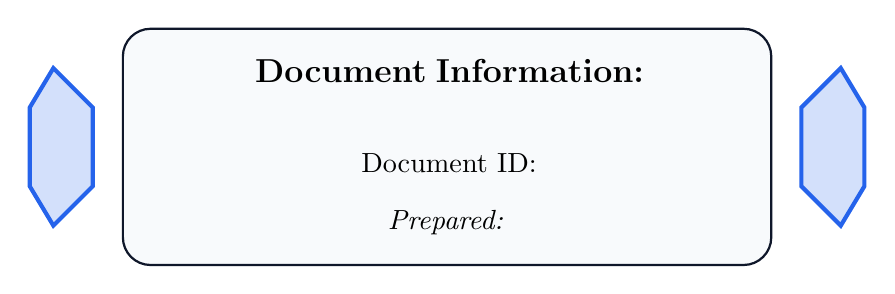
\begin{tikzpicture}
    \node[draw=primary,thick,rounded corners=10pt,fill=background,text width=8cm,align=center,minimum height=3cm] {
        \textbf{\large Document Information:}\\[0.3cm]
        \textbf{\AuthorPlaceholder}\\
        Document ID: \DocumentIDPlaceholder\\[0.3cm]
        \textit{Prepared: \DatePlaceholder}
    };
    
    % Decorative side elements
    \begin{scope}[shift={(-5,0)}]
        \draw[line width=1.5pt,accent,fill=accent!20] 
            (0,-1) -- (0.5,-0.5) -- (0.5,0.5) -- (0,1) -- (-0.3,0.5) -- (-0.3,-0.5) -- cycle;
    \end{scope}
    \begin{scope}[shift={(5,0)}]
        \draw[line width=1.5pt,accent,fill=accent!20] 
            (0,-1) -- (-0.5,-0.5) -- (-0.5,0.5) -- (0,1) -- (0.3,0.5) -- (0.3,-0.5) -- cycle;
    \end{scope}
\end{tikzpicture}
\end{center}

\vspace{1cm}

% Classification Information
\begin{center}
\begin{tabularx}{0.85\textwidth}{|X|X|}
\hline
\multicolumn{2}{|c|}{\cellcolor{primary!20}\textbf{\large Document Details}} \\
\hline
\textbf{Classification:} & \textbf{Version:} \\
\ClassificationPlaceholder & \VersionPlaceholder \\
\hline
\textbf{Distribution:} & \textbf{Status:} \\
\DistributionPlaceholder & \StatusPlaceholder \\
\hline
\end{tabularx}
\end{center}

\vfill

% Footer with elegant frame
\begin{center}
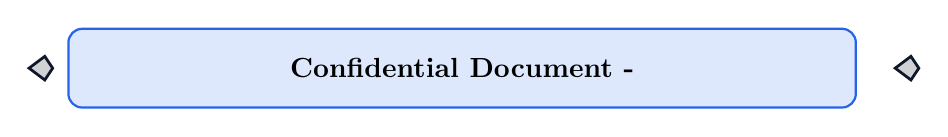
\begin{tikzpicture}
    \node[draw=accent,thick,fill=accent!15,rounded corners=5pt,minimum width=10cm,minimum height=1cm] 
        {\textbf{Confidential Document - \CompanyPlaceholder}};
    
    % Corner decorations
    \foreach \x in {-5.5, 5.5} {
        \begin{scope}[shift={(\x,0)}]
            \draw[line width=1pt,primary,fill=primary!20] 
                (0,0) -- (0.2,0.15) -- (0.3,0) -- (0.2,-0.15) -- cycle;
        \end{scope}
    }
\end{tikzpicture}
\end{center}

\vspace{1cm}
        }{}
        \ifthenelse{\equal{\UseCover}{cover9}}{
            \typeout{^^J DEBUG: Loading cover9.tex ^^J}
            % ========== COVER9: MODERN MINIMALIST DESIGN ==========
% Cover-specific dependencies
\usetikzlibrary{positioning,shapes.geometric}

% Clean, minimalist layout with simple geometric elements
\vspace{1cm}

% Institutional Information
\begin{center}
{\Large\textbf{\CompanyPlaceholder}}\\[0.3cm]
{\large \DepartmentPlaceholder}\\[0.2cm]
{\normalsize Research \& Development Division}
\end{center}

\vspace{1.5cm}

% Document Type with simple colored background
\begin{center}
\colorbox{primary}{\textcolor{white}{\Large\textbf{\quad \SubtitlePlaceholder \quad}}}
\end{center}

\vspace{2cm}

% Project Title - clean and bold
\begin{center}
{\Huge\textbf{\textcolor{primary}{\TitlePlaceholder}}}
\end{center}

\vspace{2.5cm}

% Author Information - simple table format
\begin{center}
\begin{tabular}{@{}c@{}}
\textbf{\Large Document Information:}\\[0.5cm]
\textbf{\AuthorPlaceholder}\\[0.2cm]
Document ID: \DocumentIDPlaceholder\\[0.2cm]
Version: \VersionPlaceholder\\[0.5cm]
\textit{Prepared: \DatePlaceholder}
\end{tabular}
\end{center}

\vspace{1.5cm}

% Classification Information - clean layout
\begin{center}
\begin{tabular}{@{}c@{}}
\textbf{\large Classification Details:}\\[0.3cm]
\textbf{Status:} \StatusPlaceholder\\
\textbf{Distribution:} \DistributionPlaceholder\\[0.5cm]
\textbf{Contact Information:}\\
\ContactPlaceholder
\end{tabular}
\end{center}

\vfill

% Footer - simple and clean
\begin{center}
\textbf{Classification:} \ClassificationPlaceholder
\end{center}
        }{}
        \ifthenelse{\equal{\UseCover}{cover10}}{
            \typeout{^^J DEBUG: Loading cover10.tex ^^J}
            % ========== COVER10: CONTEMPORARY BLOCKS DESIGN ==========
% Cover-specific dependencies
\usetikzlibrary{positioning,shapes.geometric}

% Top colored blocks using brand colors
\begin{tikzpicture}[remember picture,overlay]
\fill[primary] ([yshift=-0.5cm]current page.north west) rectangle ++(5cm,-1.5cm);
\fill[accent] ([xshift=5cm,yshift=-0.5cm]current page.north west) rectangle ++(5cm,-1.5cm);
\fill[secondary] ([xshift=10cm,yshift=-0.5cm]current page.north west) rectangle ++(5cm,-1.5cm);
\end{tikzpicture}

\vspace{0.3cm}

% Skip logo space since we don't have logos in our system
\vspace{1cm}

% Institutional Information
\begin{center}
{\LARGE\textbf{\CompanyPlaceholder}}\\[0.3cm]
{\Large \DepartmentPlaceholder}\\[0.2cm]
{\large Research \& Development Division}
\end{center}

\vspace{1cm}

% Document Type in Block
\begin{center}

\begin{tikzpicture}
\node[rectangle, fill=primary, text=white, minimum width=10cm, minimum height=1.5cm] 
     {\Large\textbf{\SubtitlePlaceholder}};
\end{tikzpicture}
\end{center}

\vspace{1.5cm}

% Project Title in styled box
\begin{center}
\begin{tcolorbox}[colback=background,colframe=textgray,width=0.9\textwidth,boxrule=2pt]
\begin{center}
{\LARGE\textbf{\TitlePlaceholder}}
\end{center}
\end{tcolorbox}
\end{center}

\vspace{1.5cm}

% Document Information in Grid
\begin{center}
\textbf{\Large Document Details:}\\[0.5cm]
\begin{tabular}{|c|c|}
\hline
\rowcolor{primary!20}
\textbf{Field} & \textbf{Value} \\
\hline
Author & \AuthorPlaceholder \\
\hline
Document ID & \DocumentIDPlaceholder \\
\hline
Version & \VersionPlaceholder \\
\hline
Date & \DatePlaceholder \\
\hline
\end{tabular}\\[0.5cm]
\textit{\large Status: \StatusPlaceholder}
\end{center}

\vspace{1cm}

% Classification Information in Blocks
\begin{center}
\begin{tabular}{cc}
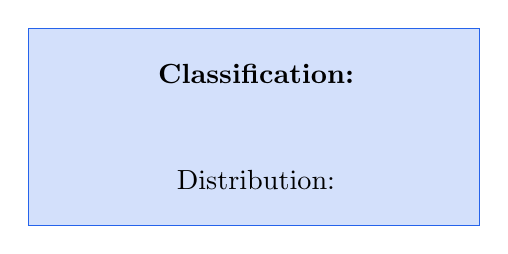
\begin{tikzpicture}
\node[rectangle, fill=accent!20, draw=accent, text width=5.5cm, align=center, minimum height=2.5cm] {
\textbf{Classification:}\\[0.2cm]
\textbf{\ClassificationPlaceholder}\\[0.3cm]
Distribution: \DistributionPlaceholder
};
\end{tikzpicture}
&
\quad

\begin{tikzpicture}
\node[rectangle, fill=secondary!20, draw=secondary, text width=5.5cm, align=center, minimum height=2.5cm] {
\textbf{Contact Information:}\\[0.2cm]
\textbf{\ContactPlaceholder}\\[0.3cm]
Company: \CompanyPlaceholder
};
\end{tikzpicture}
\end{tabular}
\end{center}

\vfill

% Footer with colored background
\begin{center}
\colorbox{textgray}{\textcolor{white}{\textbf{\quad \CompanyPlaceholder\ - \ClassificationPlaceholder\ Document \quad}}}
\end{center}
        }{}
        \end{titlepage}
        \newpage
    \else
        \typeout{^^J DEBUG: UseCover is NOT defined ^^J}
        % DEFAULT MODE: Use basic LaTeX title page
        % This creates a simple, centered title page using \maketitle
        \maketitle
    \fi
\fi

% ========== DOCUMENT CONTENT BEGINS HERE ==========
% This info box demonstrates that the Boxes module is working
\begin{infobox}[title=Performance Optimization]
This document demonstrates selective module loading. Only the features actually used are loaded, reducing compilation time while maintaining full functionality where needed.
\end{infobox}

% ========== LOAD CONTENT SECTIONS ==========
% ========== INTRODUCTION SECTION ==========
\section{Advanced Typography}

\lettrine[lines=3]{T}{his} document demonstrates advanced typography features including drop caps, enhanced spacing, and professional text formatting.

Here we show \brandname{Company Name} and \productname{Product Name} with proper letter spacing.

% ========== MATHEMATICS SECTION ==========
\subsection{Mathematical Content}

Since we enabled mathematics, we can use advanced equations:

\begin{align}
E &= mc^2 \\
F &= G\frac{m_1 m_2}{r^2} \\
\nabla \times \vec{E} &= -\frac{\partial \vec{B}}{\partial t}
\end{align}

We can also format units properly: \SI{42}{\kilo\watt\hour} and \SI{1.25}{\USD}.

% ========== TABLES SECTION ==========
\section{Professional Tables}

\begin{table}[htbp]
\caption{Performance Comparison}
\centering
\rowcolors{2}{rowalt}{white}
\begin{tabularx}{\textwidth}{L{3cm}C{3cm}R{2cm}X}
\rowcolor{headerbg}
\textcolor{headertext}{\textbf{Configuration}} &
\textcolor{headertext}{\textbf{Compile Time}} &
\textcolor{headertext}{\textbf{Memory}} &
\textcolor{headertext}{\textbf{Features}} \\
\toprule
Original config.tex & 45-60s & High & All features \\
Core only & 8-12s & Low & Basic features \\
Selective modules & 15-25s & Medium & Selected features \\
\bottomrule
\end{tabularx}
\end{table}

% ========== CONCLUSION SECTION ==========
\section{Conclusion}

This modular approach allows you to:
\begin{itemize}
    \item Reduce compilation time significantly
    \item Use only needed features
    \item Maintain compatibility with Overleaf free plan
    \item Keep full functionality when required
\end{itemize}

\begin{alertbox}
\textbf{Important:} Only enable modules you actually need in your document to maintain optimal performance on Overleaf's free plan.
\end{alertbox}


\end{document}
